% A pure minimalistic LaTeX-Beamer theme for everyone to use.
% Copyright (C) 2020 Kai Norman Clasen
% Edited by Lucas Saldyt

\documentclass[aspectratio=169]{beamer}
\DeclareMathSizes{12}{30}{16}{12}
% should also look nice for the classic aspectratio
% of course, than the text has to be refitted
% \documentclass{beamer} 
\usepackage[utf8]{inputenc}
\usepackage[T1]{fontenc}
\usepackage{tikz}
\usepackage{amsmath}
\usepackage[export]{adjustbox}

\DeclareMathOperator*{\argmin}{\arg\!\min}
\DeclareMathOperator*{\argmax}{\arg\!\max}

\usetheme[showmaxslides, darkmode]{pureminimalistic}

\usepackage[american]{babel}
\usepackage{csquotes}
\usepackage[style=apa, backend=biber]{biblatex}
\DeclareLanguageMapping{american}{american-UoN}

% \usepackage[english]{babel}
% \usepackage[backend=biber,style=apa]{biblatex}
% \DeclareLanguageMapping{english}{english-apa}
\addbibresource{sources.bib}

% this makes it possible to add backup slides, without counting them
\usepackage{appendixnumberbeamer}
\renewcommand{\appendixname}{\texorpdfstring{\translate{appendix}}{appendix}}

\renewcommand{\logotitle}{
\includegraphics[width=.2\linewidth]{logos/asu_logo_alt.png}}
\renewcommand{\logoheader}{}
\renewcommand{\logofooter}{
\includegraphics[width=.15\linewidth]{logos/asu_logo_alt.png}}
\renewcommand{\emph}[1]{{\Huge \color{pureminimalistic@text@red} #1}}

\definecolor{m1}{RGB}{30, 76, 214}
\definecolor{m2}{RGB}{161, 3, 74}
\definecolor{m3}{RGB}{255, 132, 0}
\definecolor{m4}{RGB}{255, 196, 0}
\definecolor{m5}{RGB}{3, 171, 34}
\definecolor{grey}{RGB}{130, 130, 130}

\title[Lifelong Learning for Planning]{Lifelong Learning for Robot Path-Planning}
\author{Lucas Saldyt}
\institute{Arizona State University} 
\date{\today}

\begin{document}

% Hello, I'm Lucas, and today I'll be presenting  "Lifelong Learning for Robot Path Planning"
\maketitle

\begin{frame}[plain]
  % This thesis focuses on environmental adaptation in robots.
  % An example robot is NASA's Perseverance rover, which was custom-engineered for mars.
  % Because of resource constraints and a desire for reliability, this rover doesn't use machine learning directly
  \begin{figure}
  \centering
  \vspace*{-1em}
  \hspace*{-3em}
  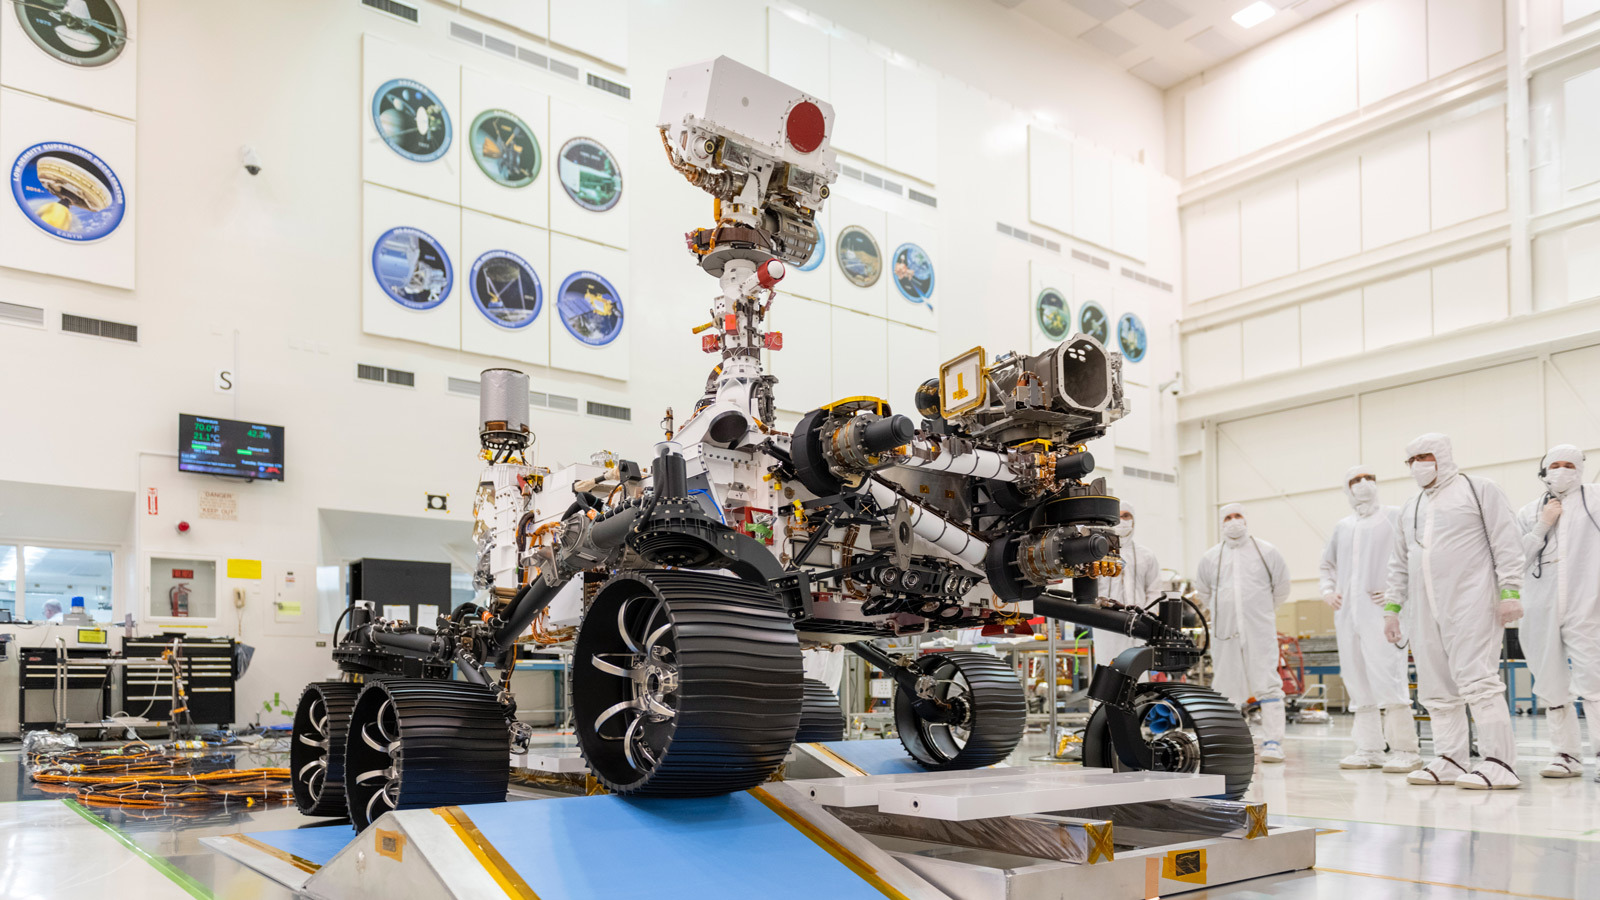
\includegraphics[height=9.5cm,keepaspectratio]{figures/perseverance.jpg}
  \end{figure}
\end{frame}

\begin{frame}[plain]
  % Instead, the rover uses an engineered navigation algorithm, or is even controlled directly.
  % As an environment, Mars offers unique challenges.
  % For example, rocks can puncture the rover's wheels and sand can trap the rover.
  % The rover relies on a combination of on-board and satellite based sensor data, which is often imperfect.
  % Also, low-latency direct human control is impossible.
  \begin{figure}
  \centering
  \vspace*{-1em}
  \hspace*{-3em}
  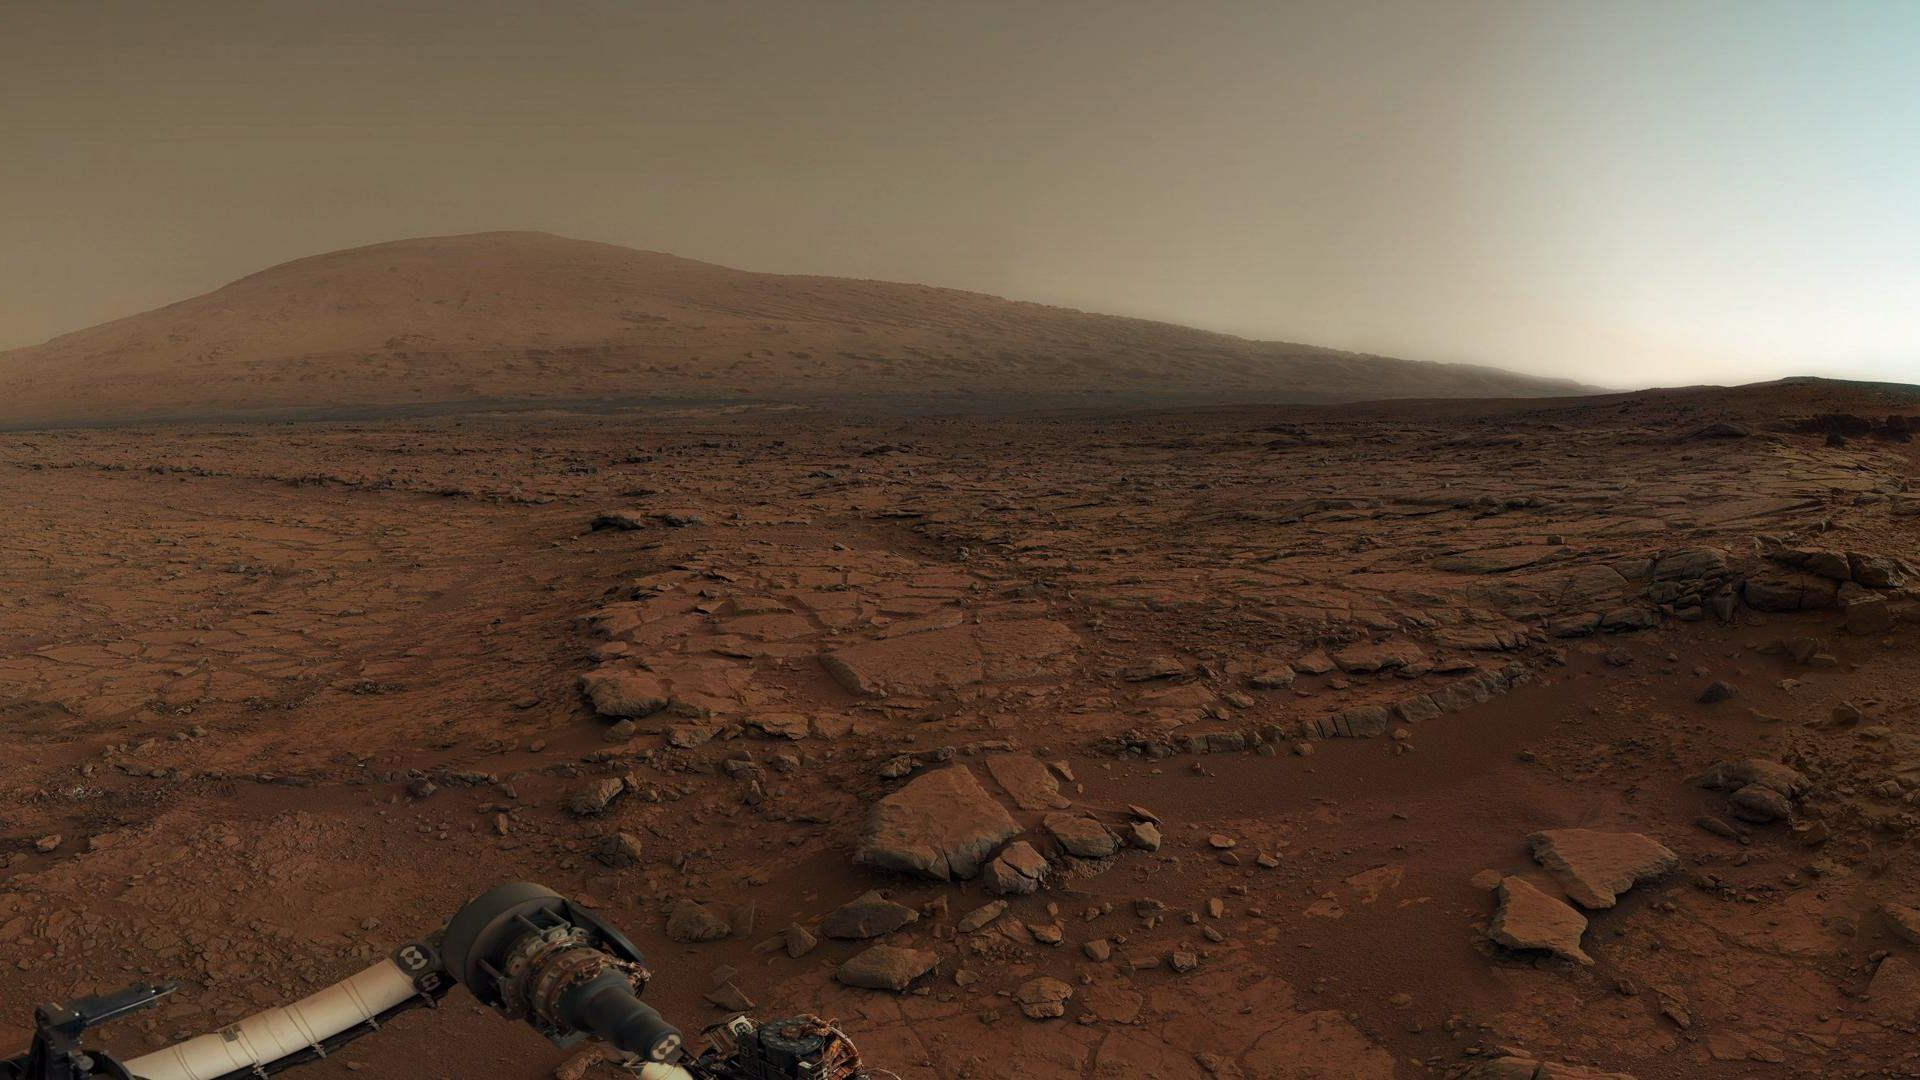
\includegraphics[height=9.5cm,keepaspectratio]{figures/mars_surface.jpg}
  \end{figure}
\end{frame}

\begin{frame}[plain]
  % Alternatively, consider an environment like an Amazon warehouse.
  % In contrast to mars, it is easy to navigate.
  % The floor is perfectly smooth, the environment is mapped almost perfectly.
  % Communication is fast, and it is easier integrate advanced machine learning algorithms with robots.
  % However, in an environment like this, there can be multiple robots, or even human-robot interaction.
  % So, robots must plan carefully to avoid dangerous collisions.
  % (pause)
  % Considering these differences two example environments brings us to the main problem of this thesis.
  \begin{figure}
  \centering
  \vspace*{-1em}
  \hspace*{-3em}
  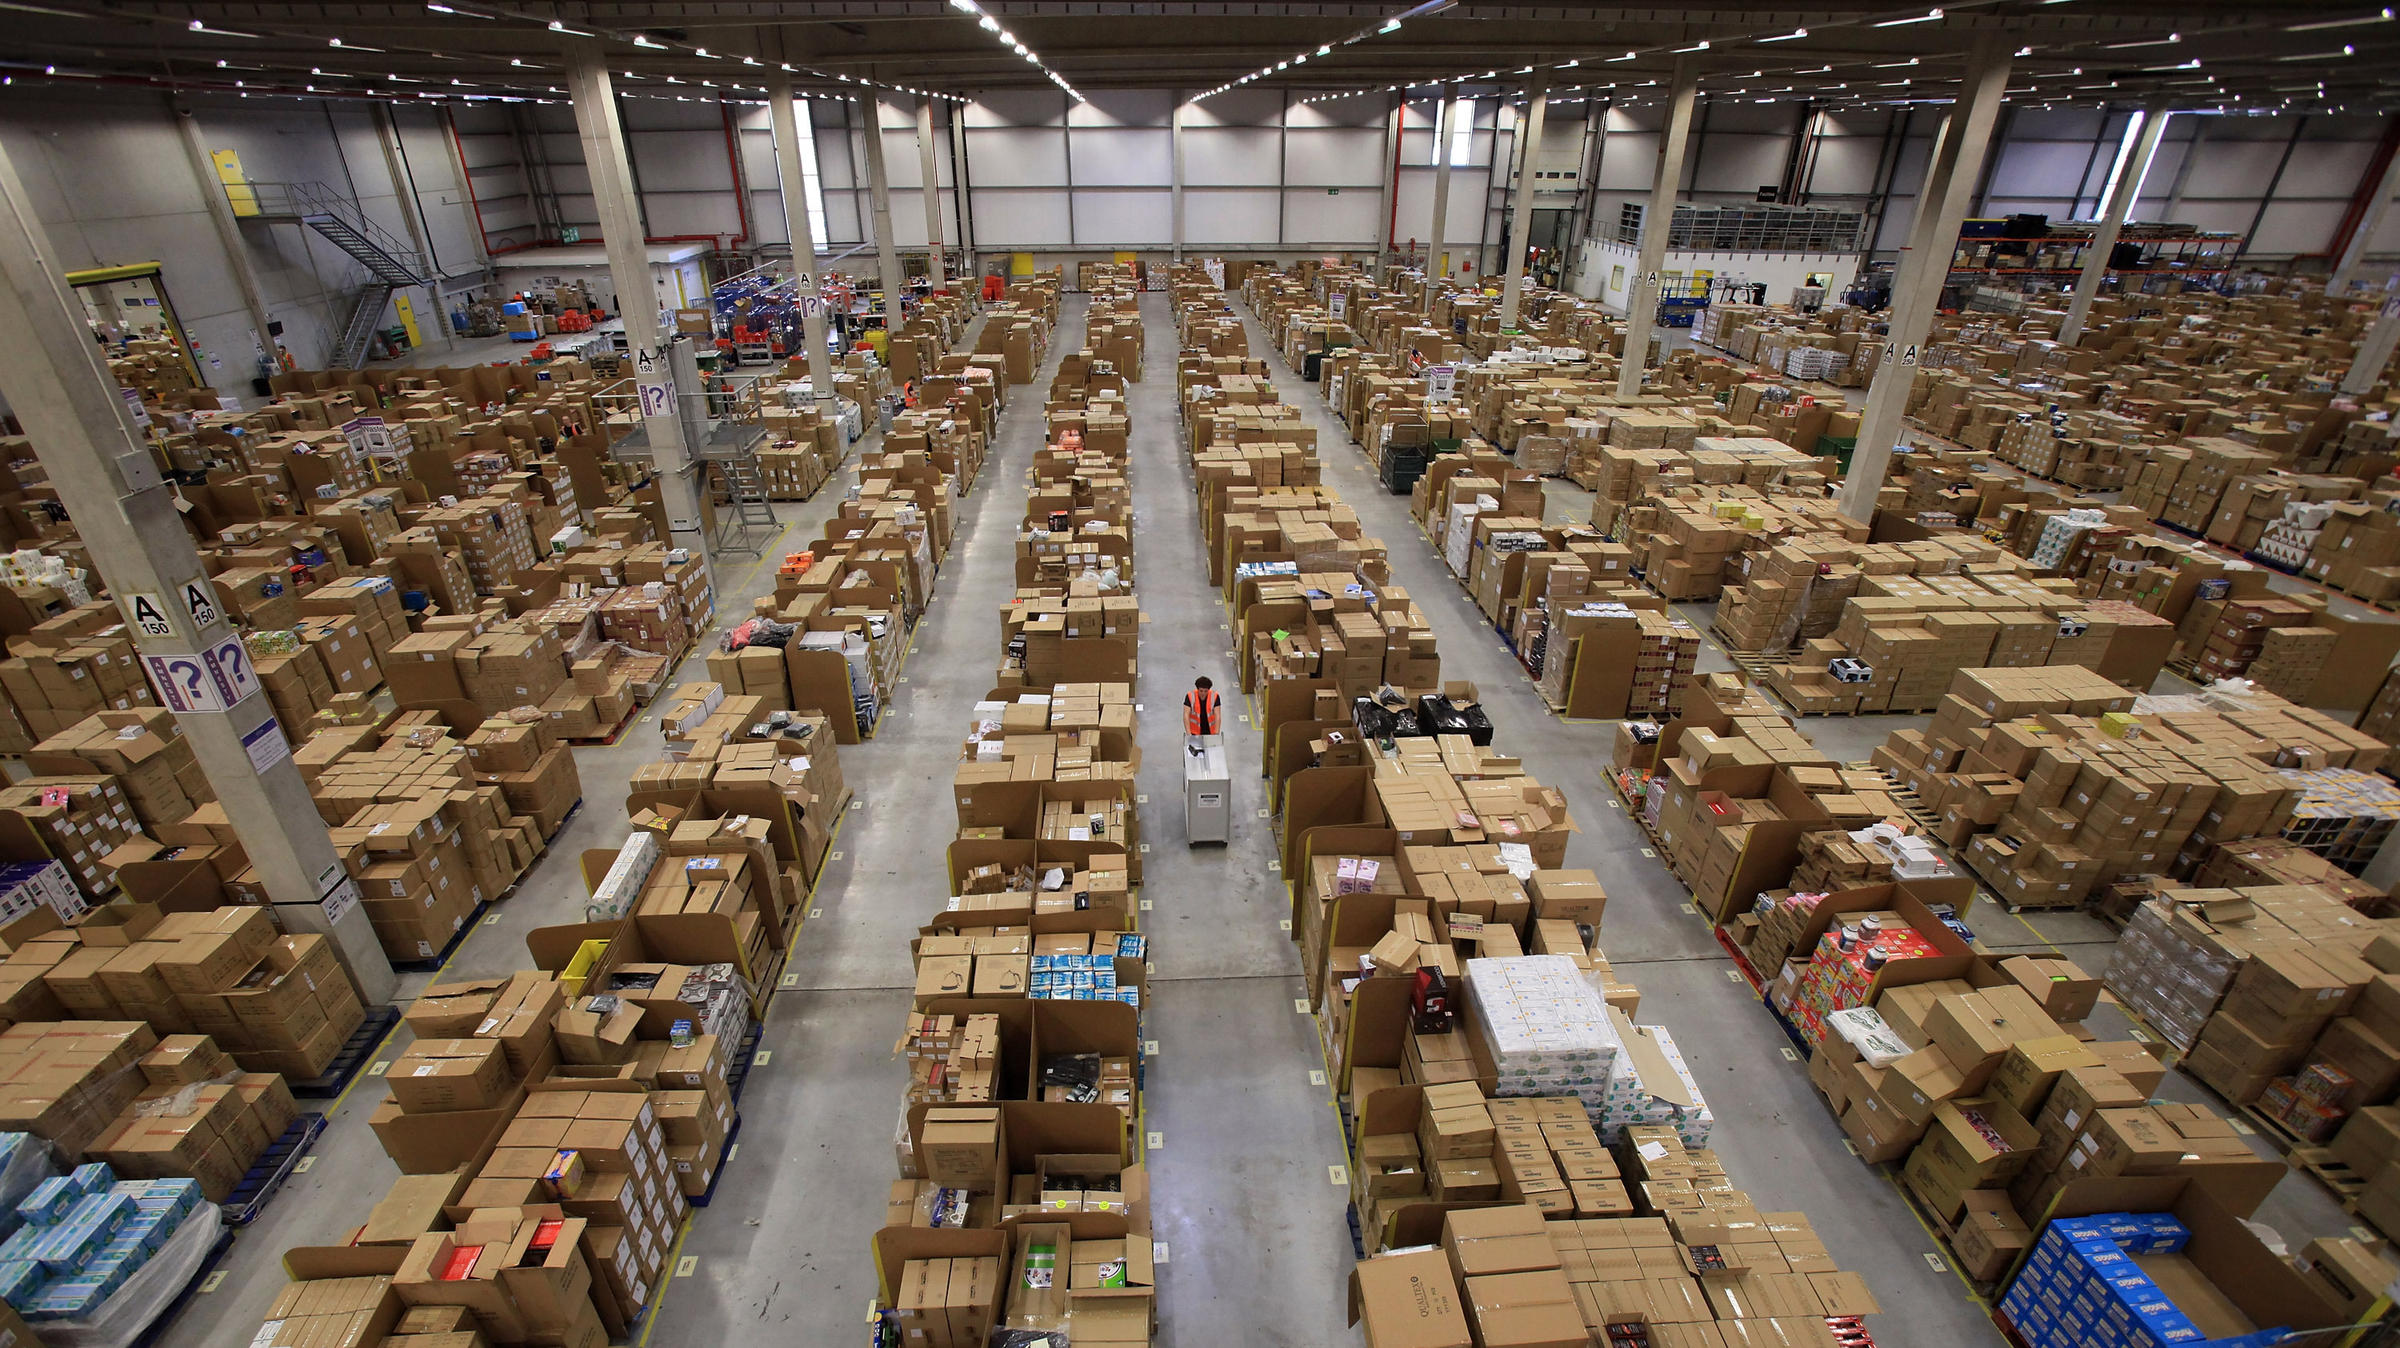
\includegraphics[height=9.5cm,keepaspectratio]{figures/warehouse.jpg}
  \end{figure}
\end{frame}

\begin{frame}{{\color{pureminimalistic@text@white} Core Goals \& Concepts}}
  % Conceptually, the focus of this thesis is on life-long robot learning.
  %   
  \begin{columns}[T]
      \begin{column}{.6\linewidth}
          \begin{vfilleditems}
            \item \emph{Learning}
              \begin{itemize}
                \item {\Medium Flexibility: adapt to new tasks}
              \end{itemize}
            \vspace{1em}
            \item \emph{Specialization}
              \begin{itemize}
                \item {\Medium Learn environment details?}
              \end{itemize}
            \vspace{1em}
            \item \emph{Generalization}
              \begin{itemize}
                \item {\Medium Learn overall task proficiency?}
              \end{itemize}
          \end{vfilleditems}
      \end{column}
      \begin{column}{.4\linewidth}
          \begin{figure}
              \centering
              \caption{Where is this image from?}
              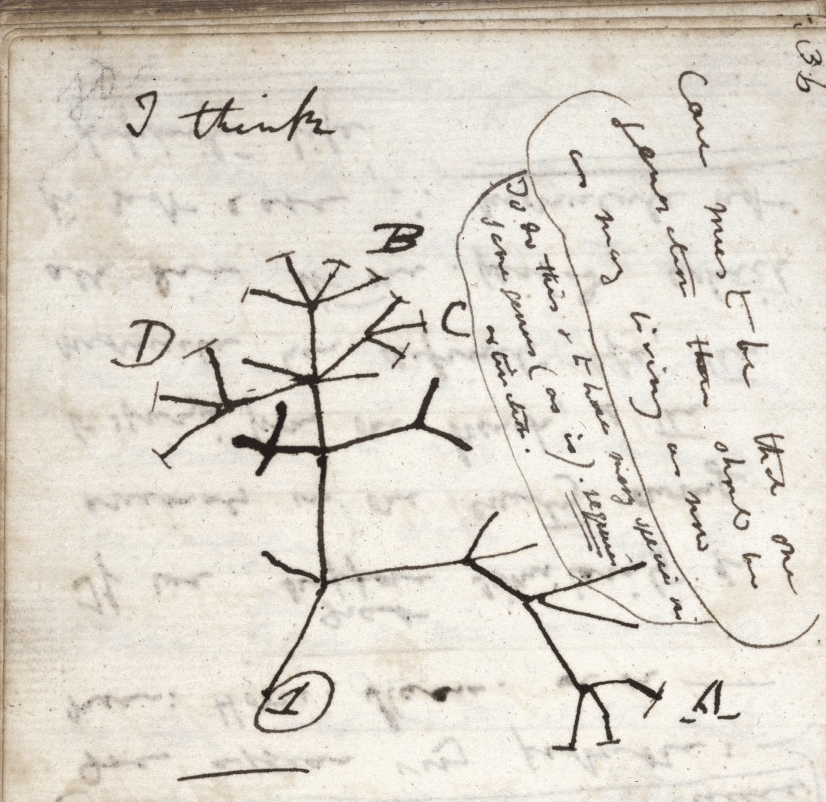
\includegraphics[height=5cm, keepaspectratio]{figures/i_think.png}
              \label{fig:my_label}
          \end{figure}
      \end{column}
  \end{columns}
\end{frame}

{
\setbeamercolor{background canvas}{bg=white}
\begin{frame}[plain]
  \begin{figure}
  \centering
  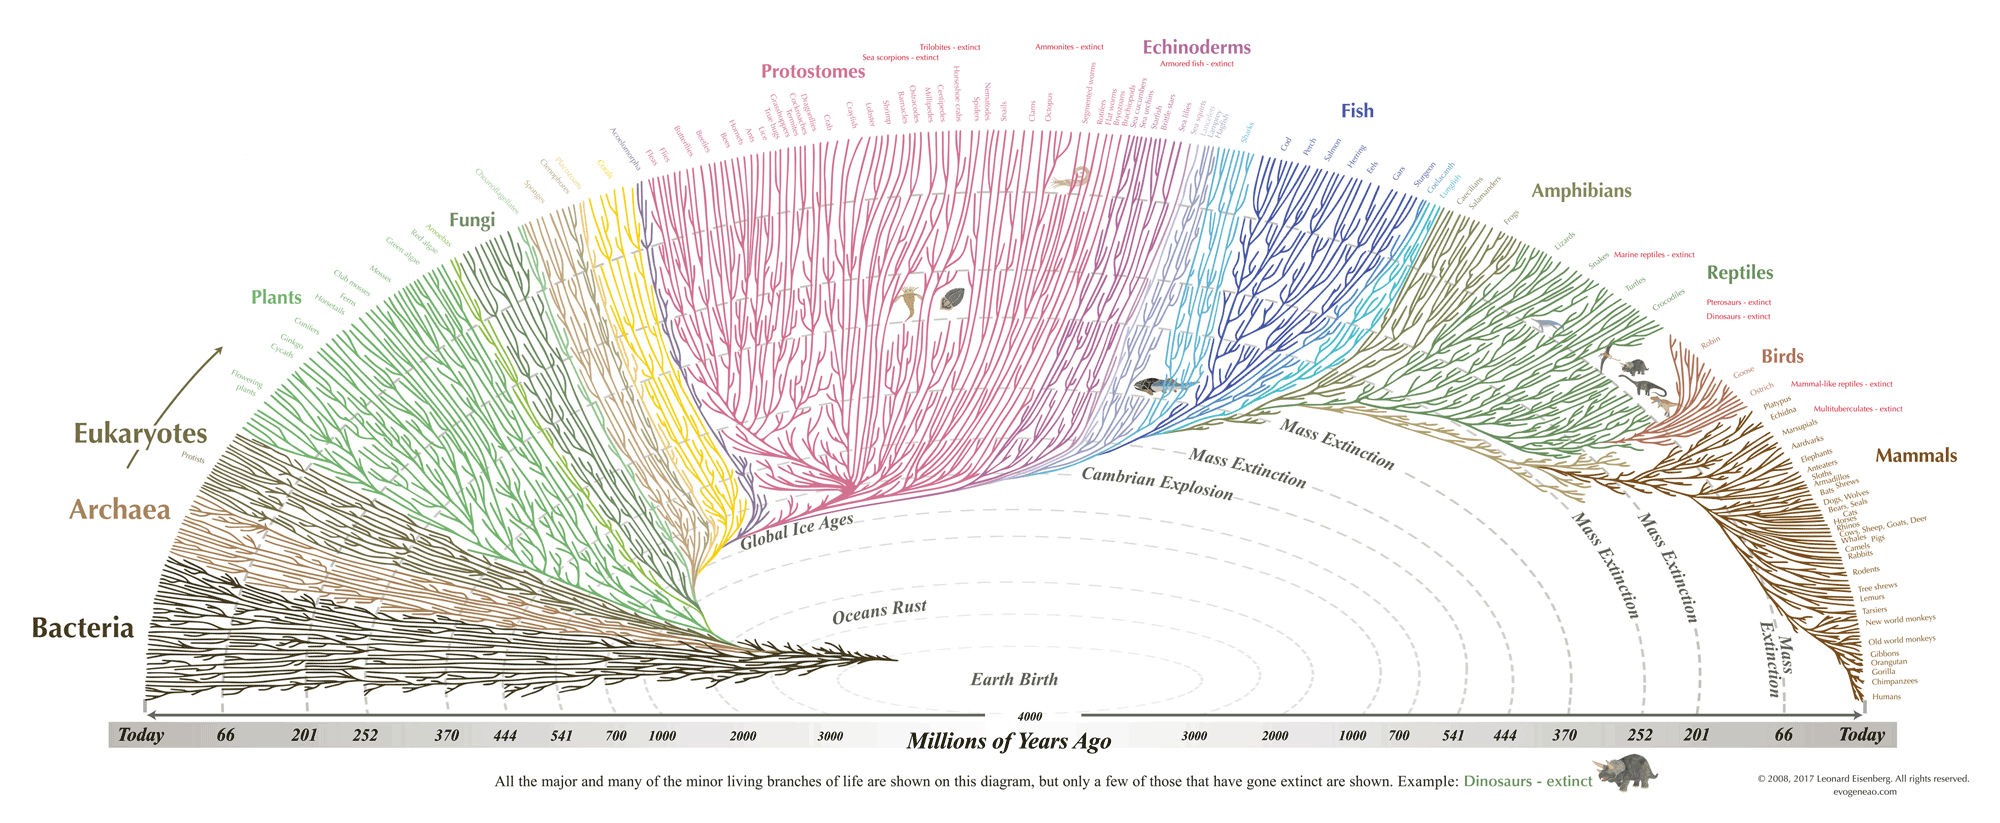
\includegraphics[width=1.0\linewidth,keepaspectratio]{figures/tree_of_life.png}
  \end{figure}
  \begin{center}
      \emph{Natural evolution}
  \end{center}
\end{frame}
}

\begin{frame}[plain]
  \begin{figure}
  \centering
  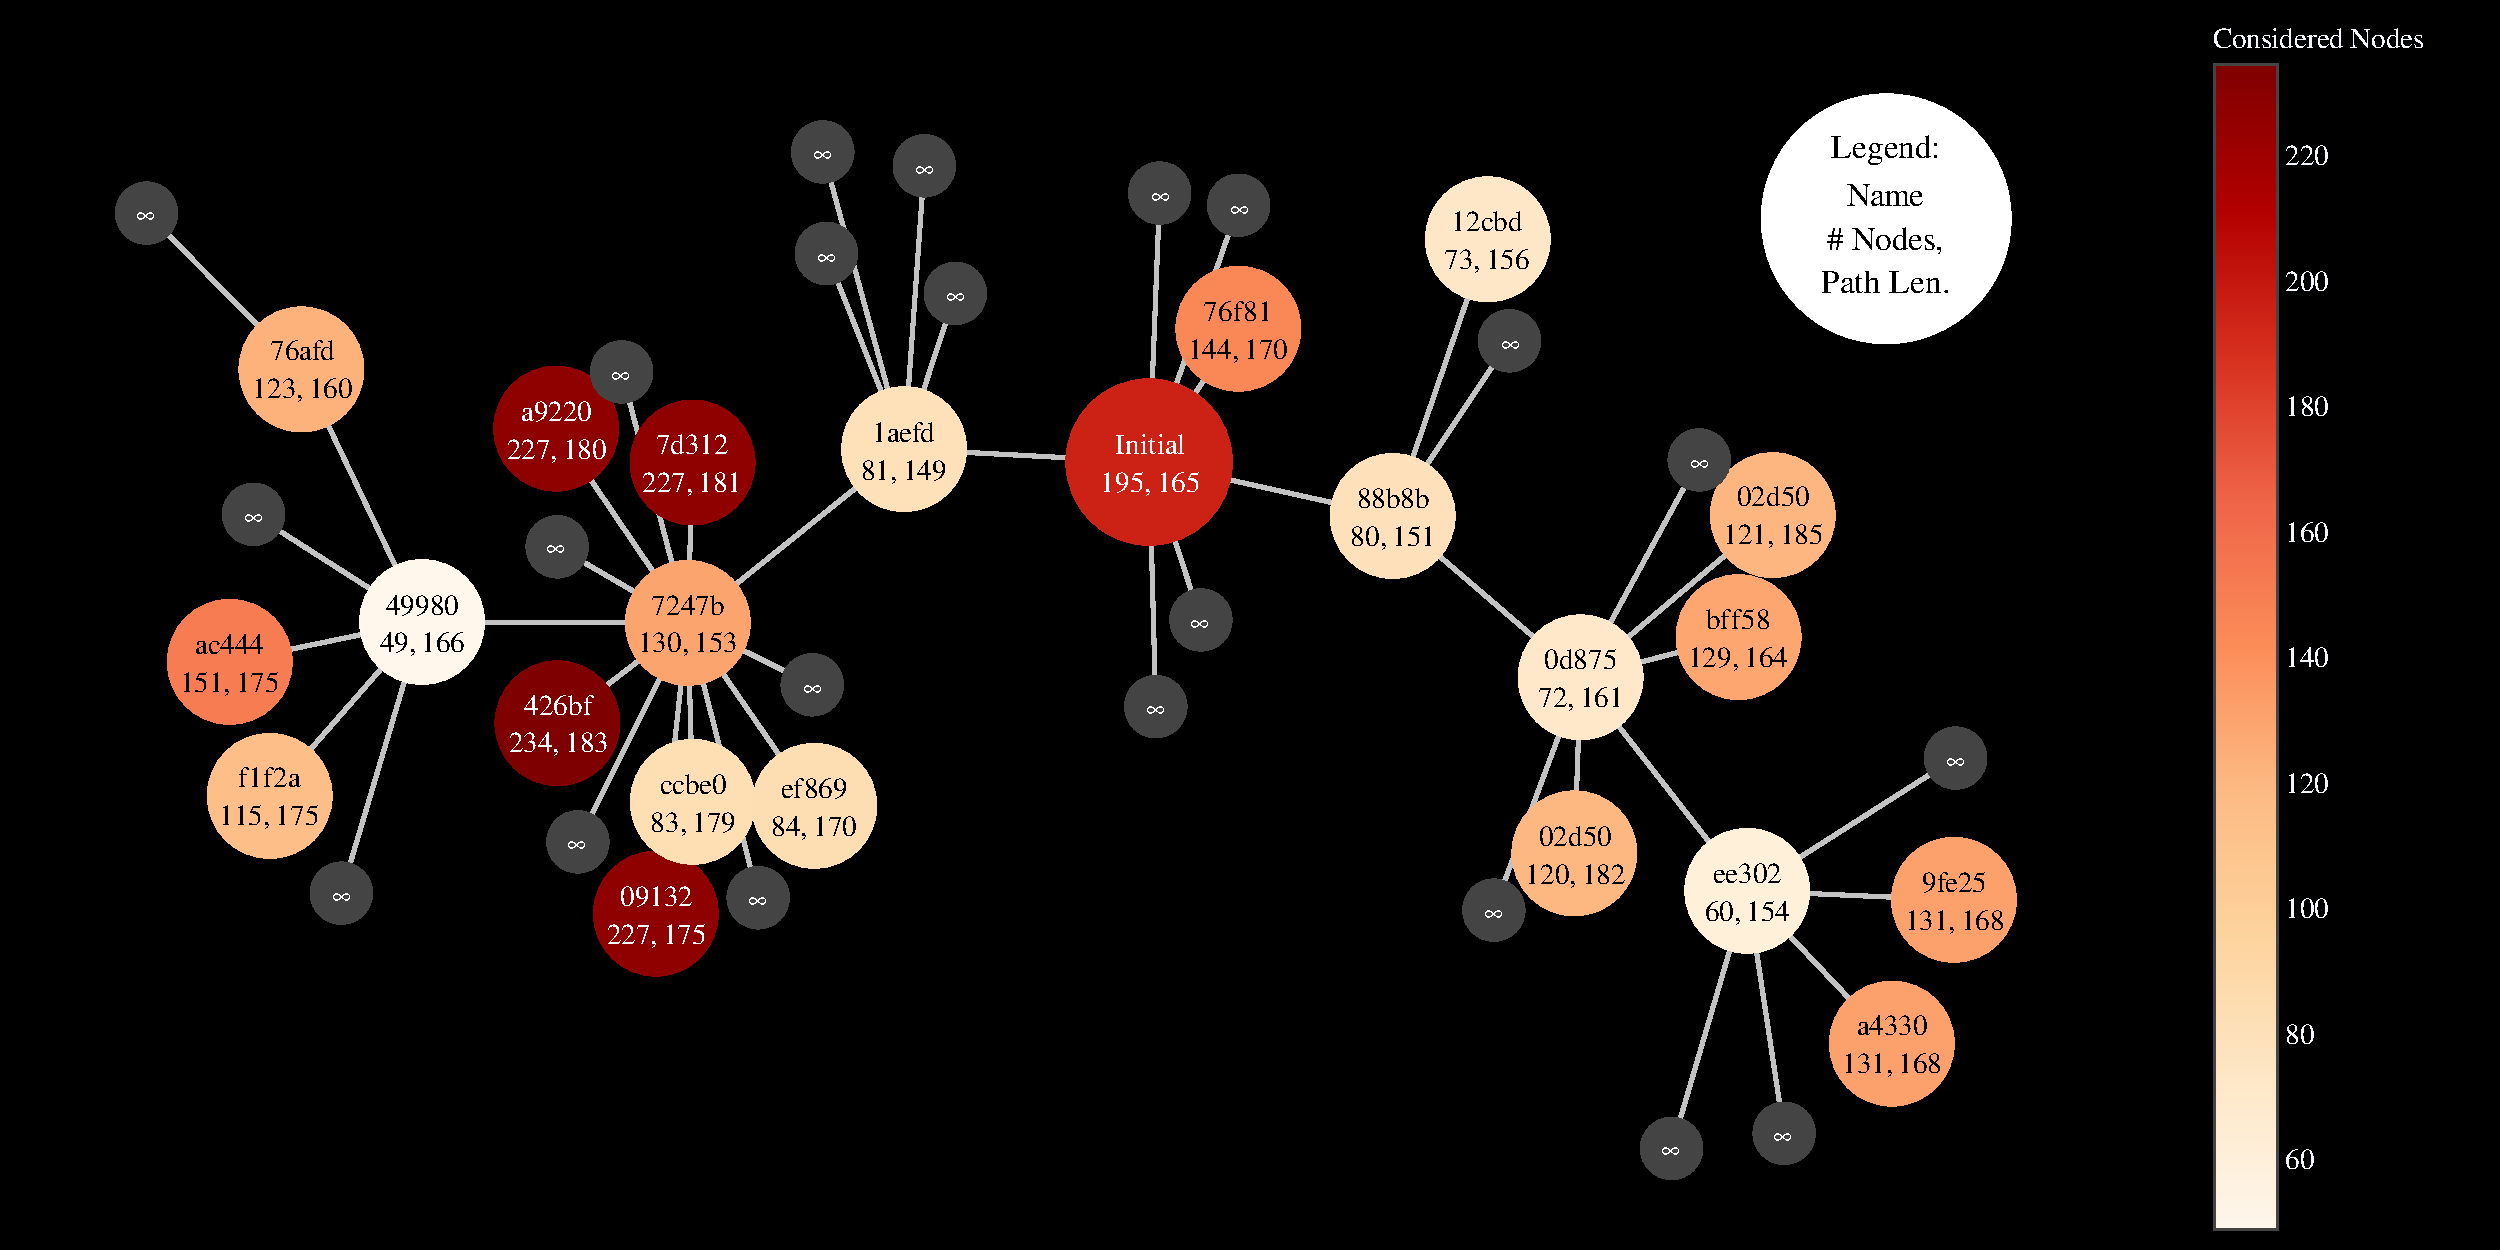
\includegraphics[width=1.0\linewidth,keepaspectratio]{figures/tree.pdf}
  \end{figure}
  \begin{center}
  \emph{Evolved Computer Programs}
  \end{center}
\end{frame}

% This thesis focuses *specifically* on path-planning.
% Originally, it focused on graph-based planning, such as A*, DFS, BFS
% However, it has moved towards sampling-based planning, such as RRT* variants.
% These are more common on real-world problems,
%   and also have more variants

\begin{frame}[plain]{Problems Considered}
  \begin{columns}[T]
      \begin{column}{.5\linewidth}
          % 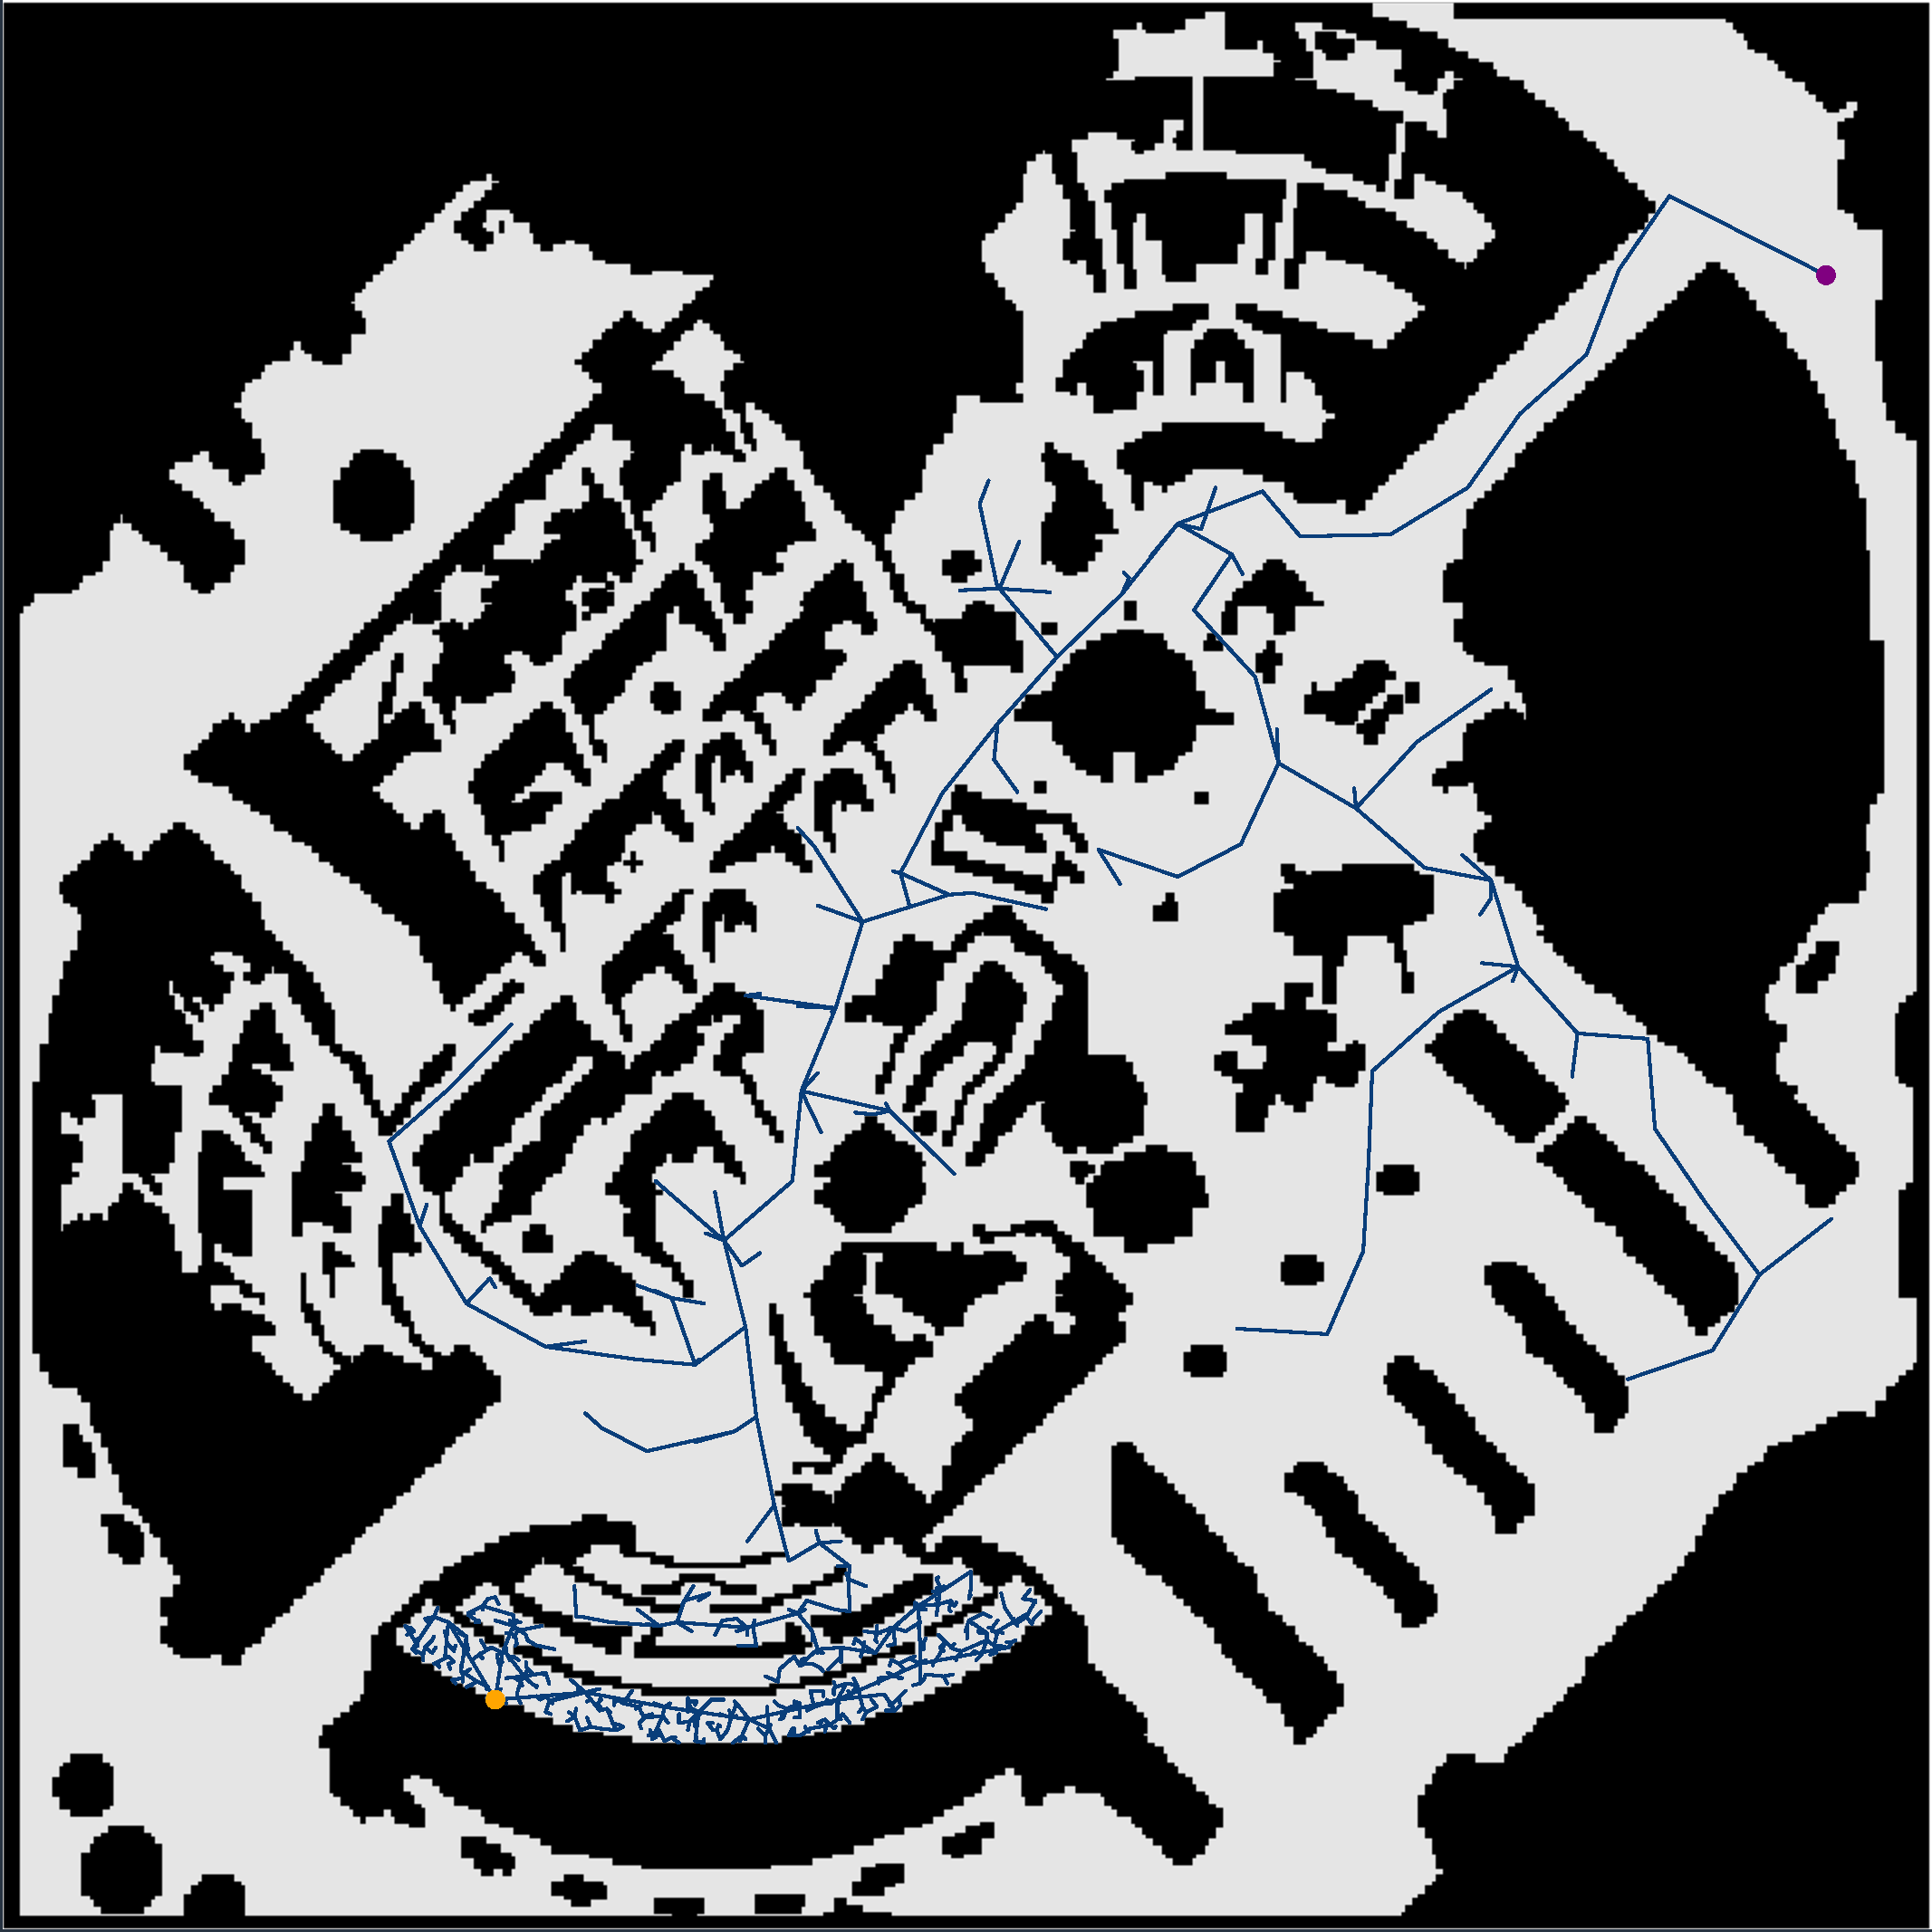
\includegraphics[width=1.0\linewidth, keepaspectratio]{figures/baldurs_rrt_one_off.pdf}
          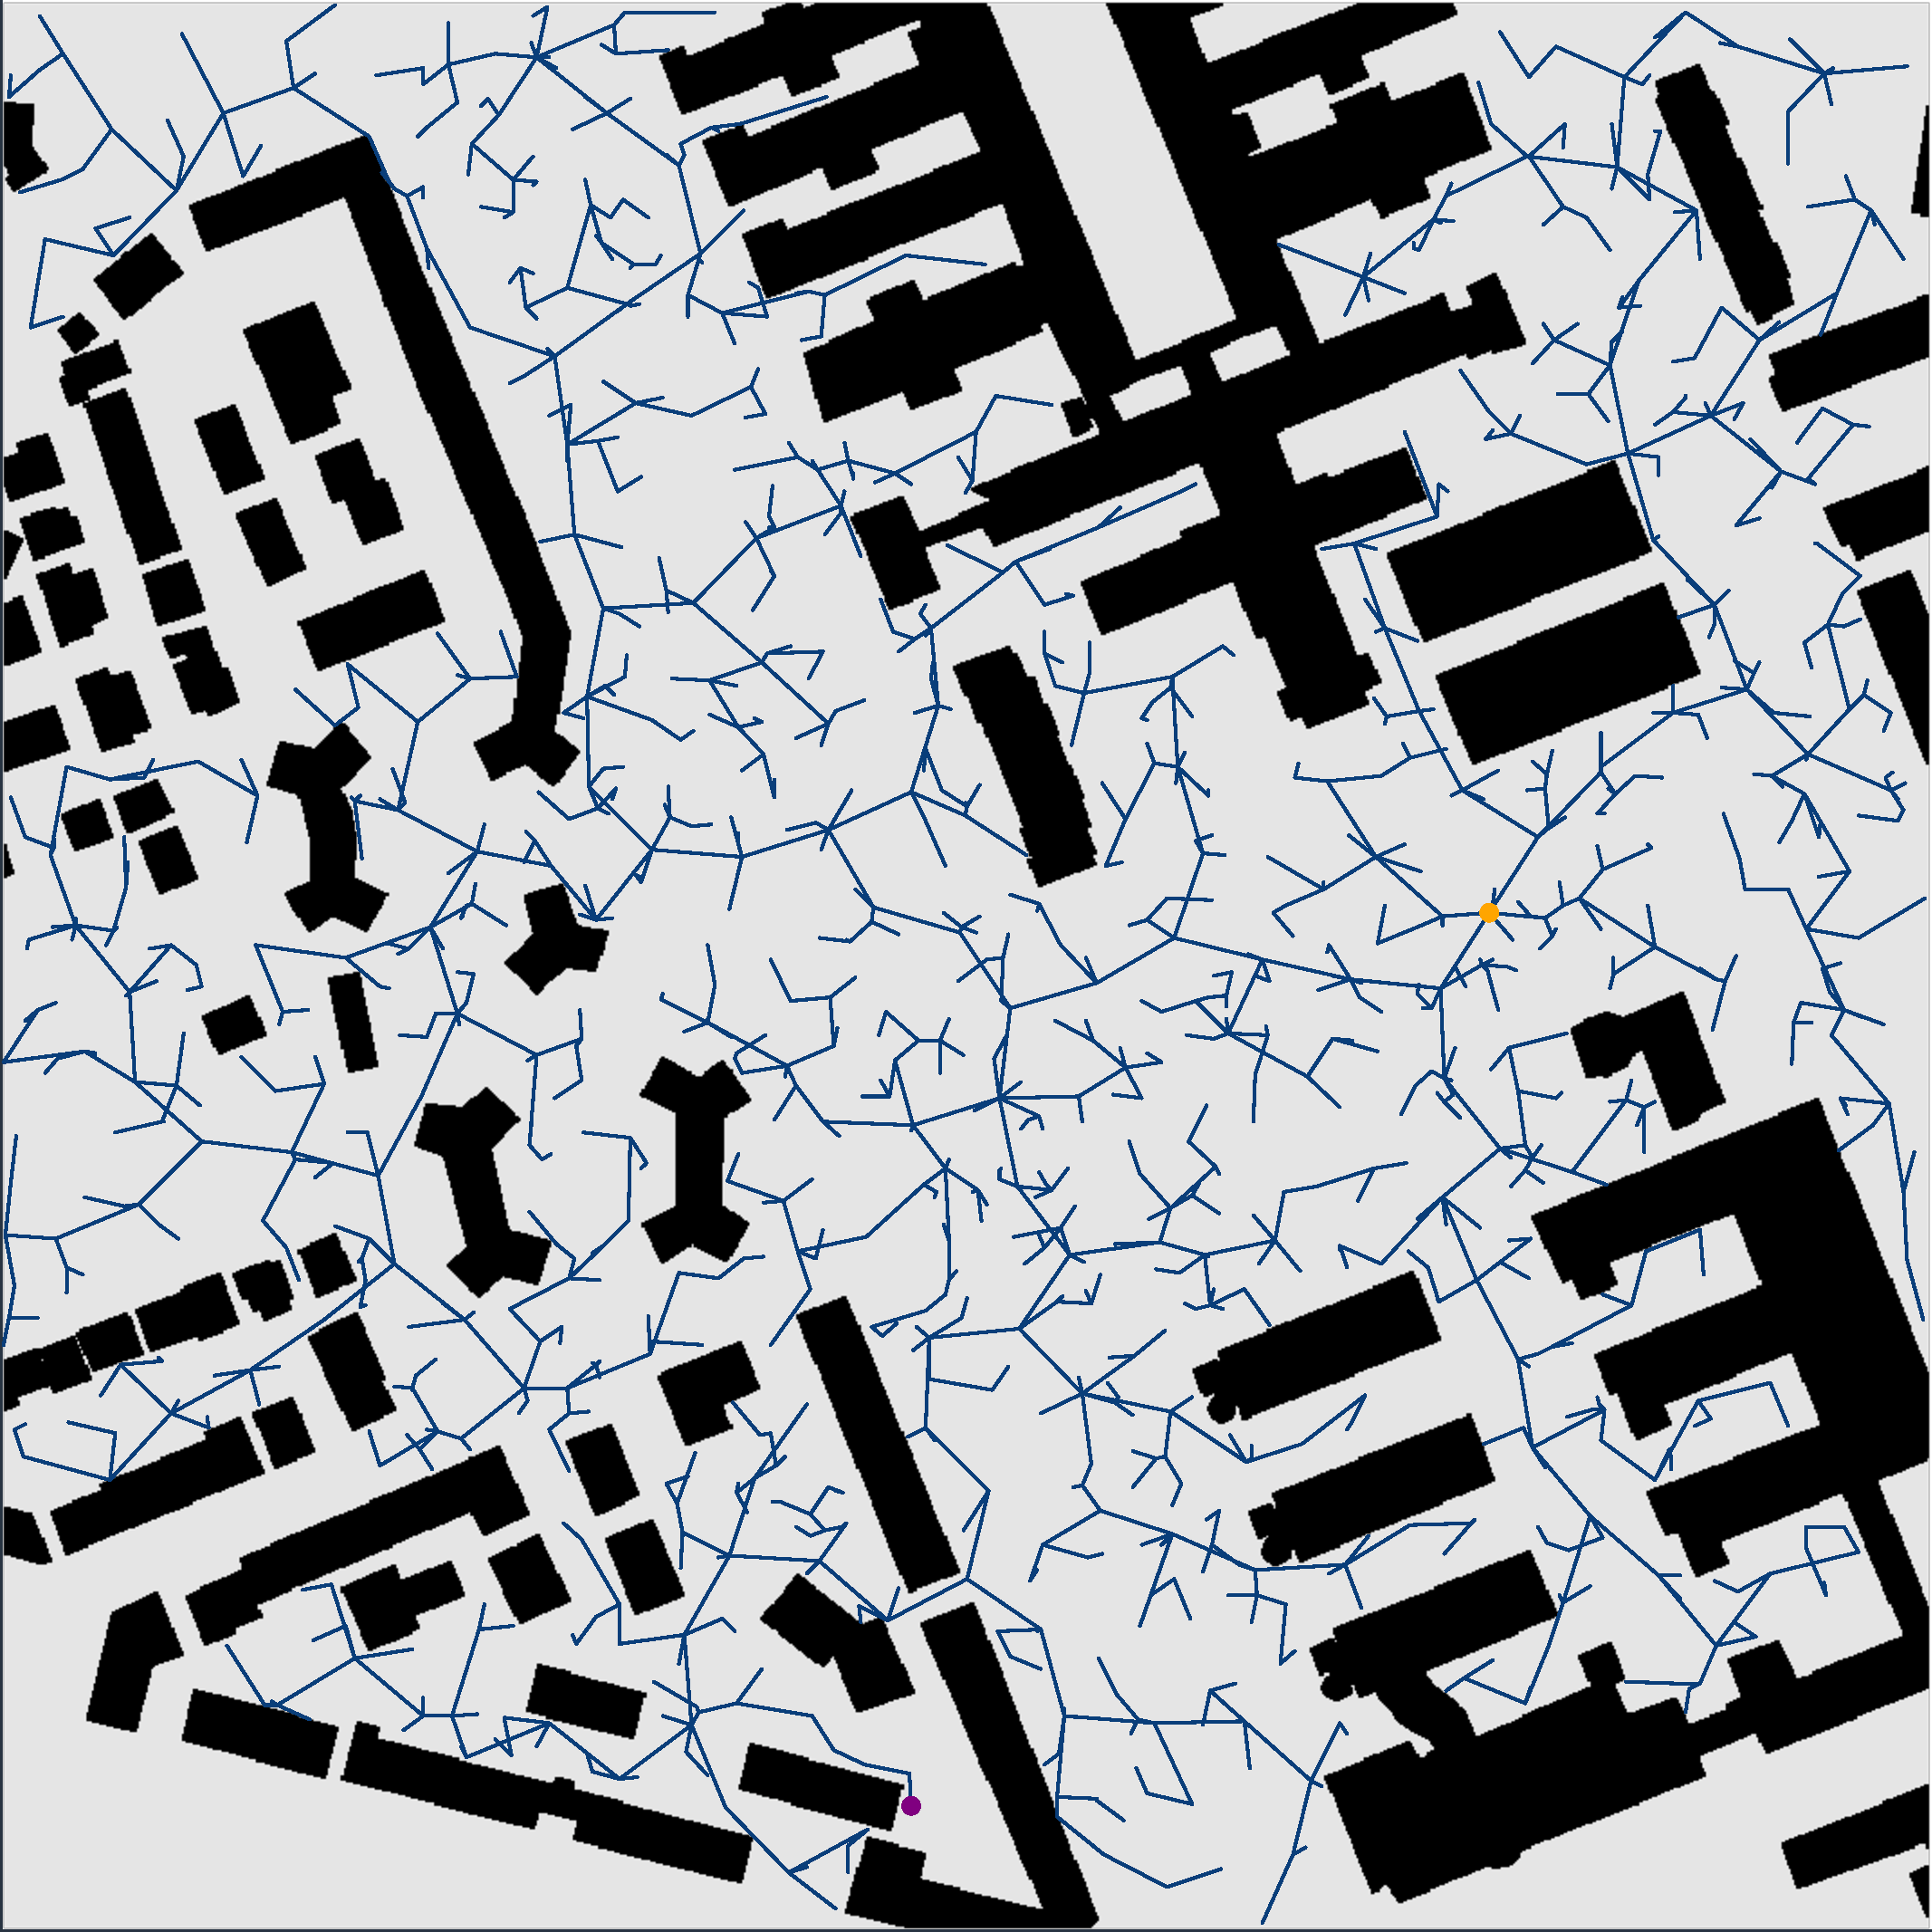
\includegraphics[width=1.0\linewidth, keepaspectratio]{figures/one_off.pdf}
      \end{column}
      \begin{column}{.5\linewidth}
          {\Huge Path Planning}
          \begin{vfilleditems}
              \item {\Large Graph-based}
              \vspace{1em}
              \item {\Large Sample-based \Medium (left)}
              \vspace{1em}
              \item {\color{grey} {\Large Dynamic}}
              \vspace{1em}
              \item {\color{grey} {\Large Multi-agent}}
          \end{vfilleditems}
          \vspace{1em}
          {\color{grey} {\Large Symbolic Regression}}
          \vspace{1em}
          {\color{grey} {\Large Neural Arch. Search}}
      \end{column}
  \end{columns}
\end{frame}

\begin{frame}[plain]{Graph-based search (New York)}
    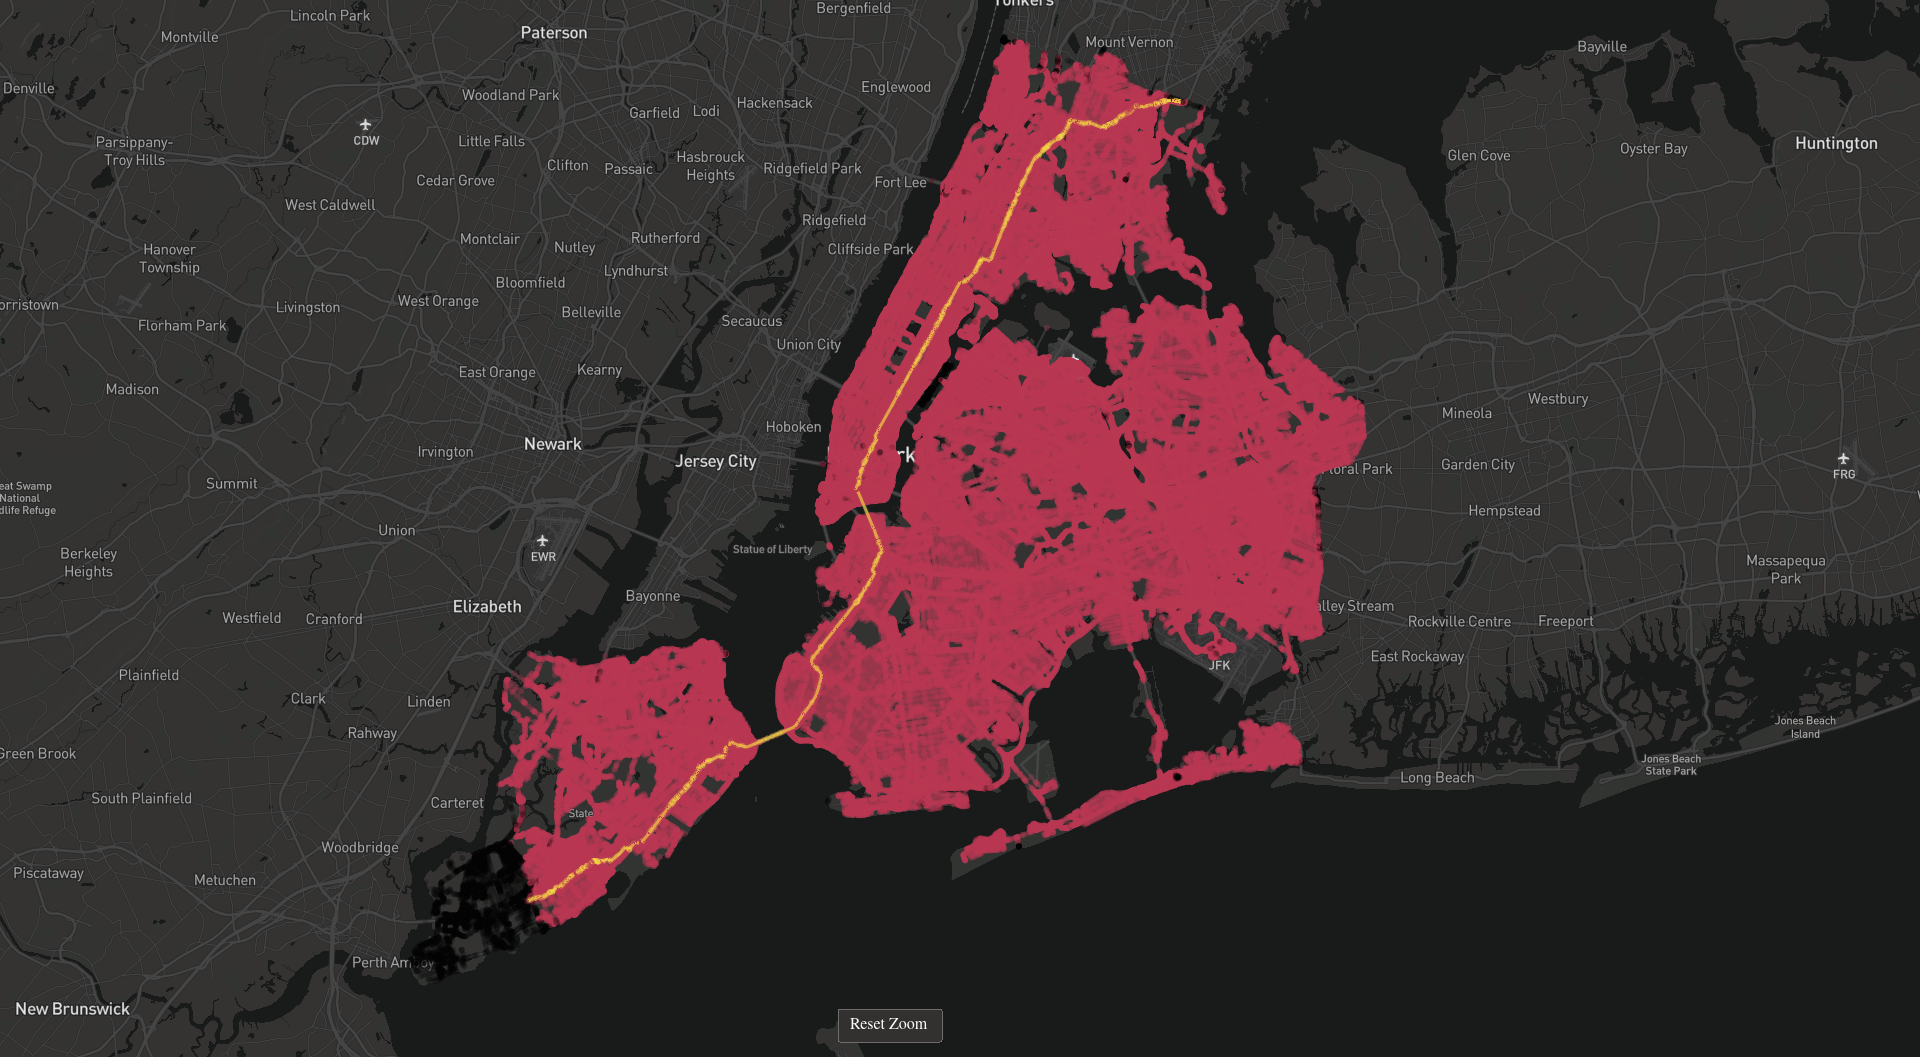
\includegraphics[width=1.0\linewidth, keepaspectratio]{figures/ny_graph_based.png}
\end{frame}

\begin{frame}[plain]{Graph-based search (New York)}
    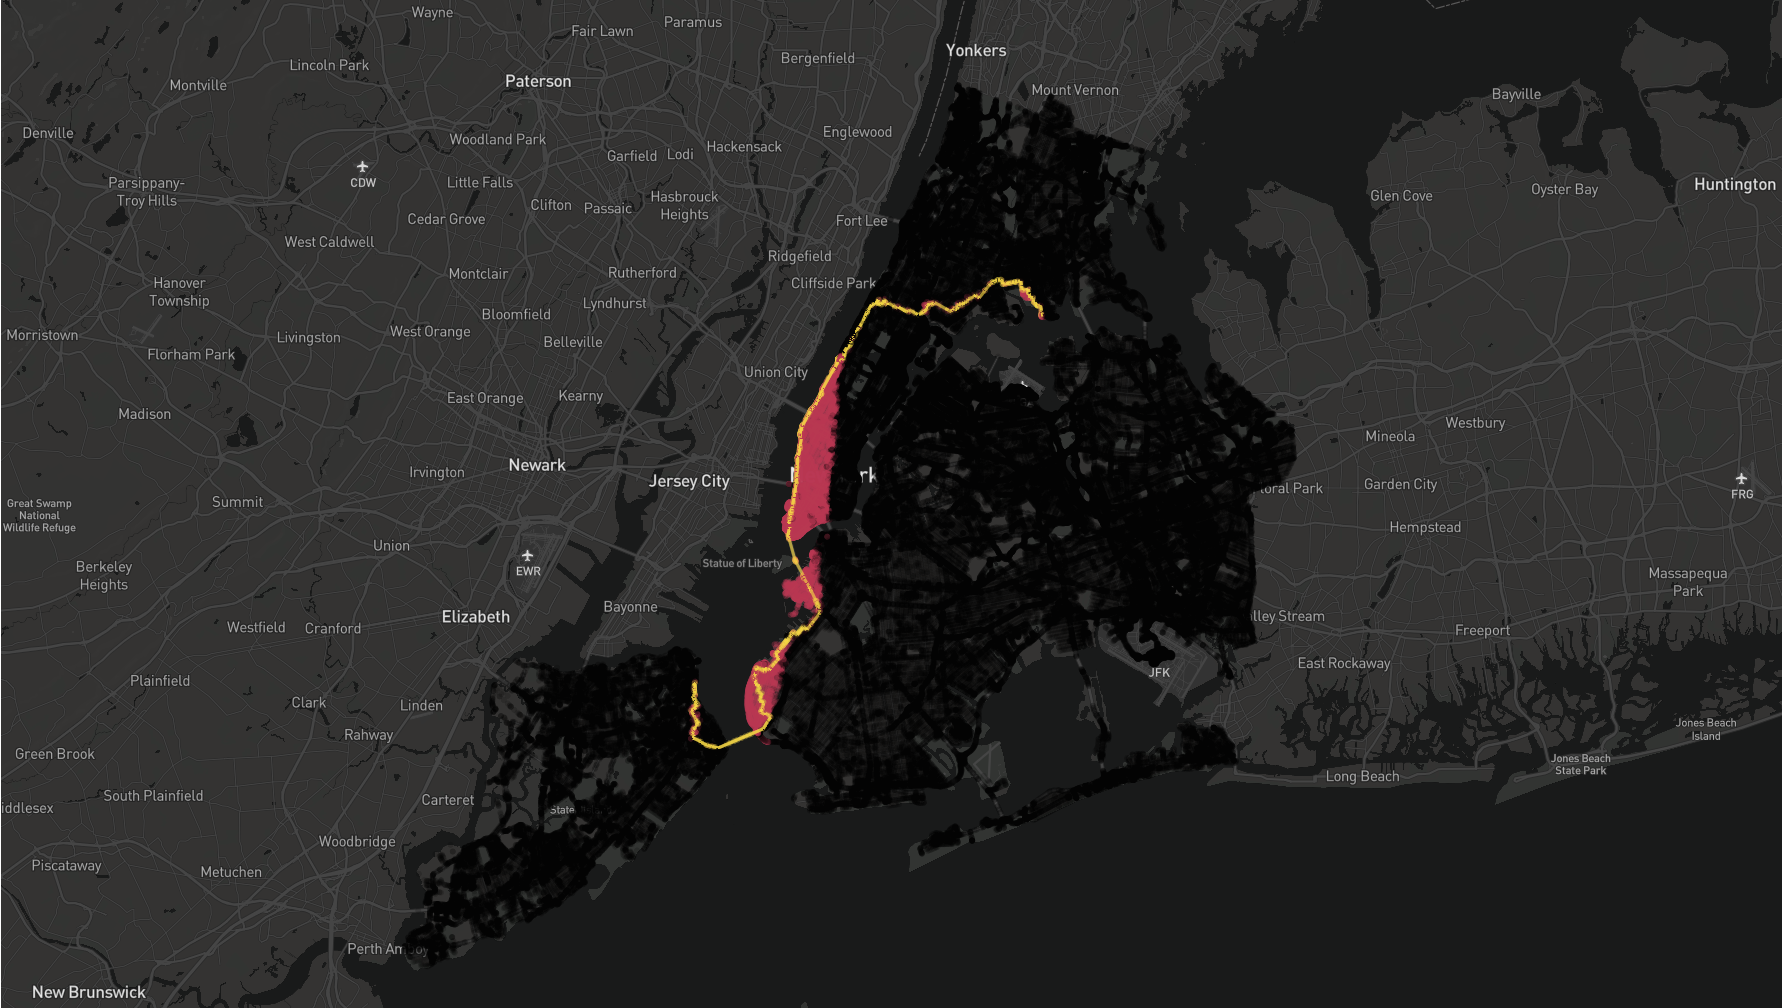
\includegraphics[width=1.0\linewidth, keepaspectratio]{figures/ny_graph_based_geodesic.png}
\end{frame}

\begin{frame}[plain]{Graph-based search (Paris)}
  \begin{columns}[T]
      \begin{column}{.4\linewidth}
          \begin{vfilleditems}
              \item {\Large Breadth-first search (BFS)}
              \item {\Large Depth-first search (DFS)}
              \item {\Large A* variants}
          \end{vfilleditems}
      \end{column}
      \begin{column}{.6\linewidth}
      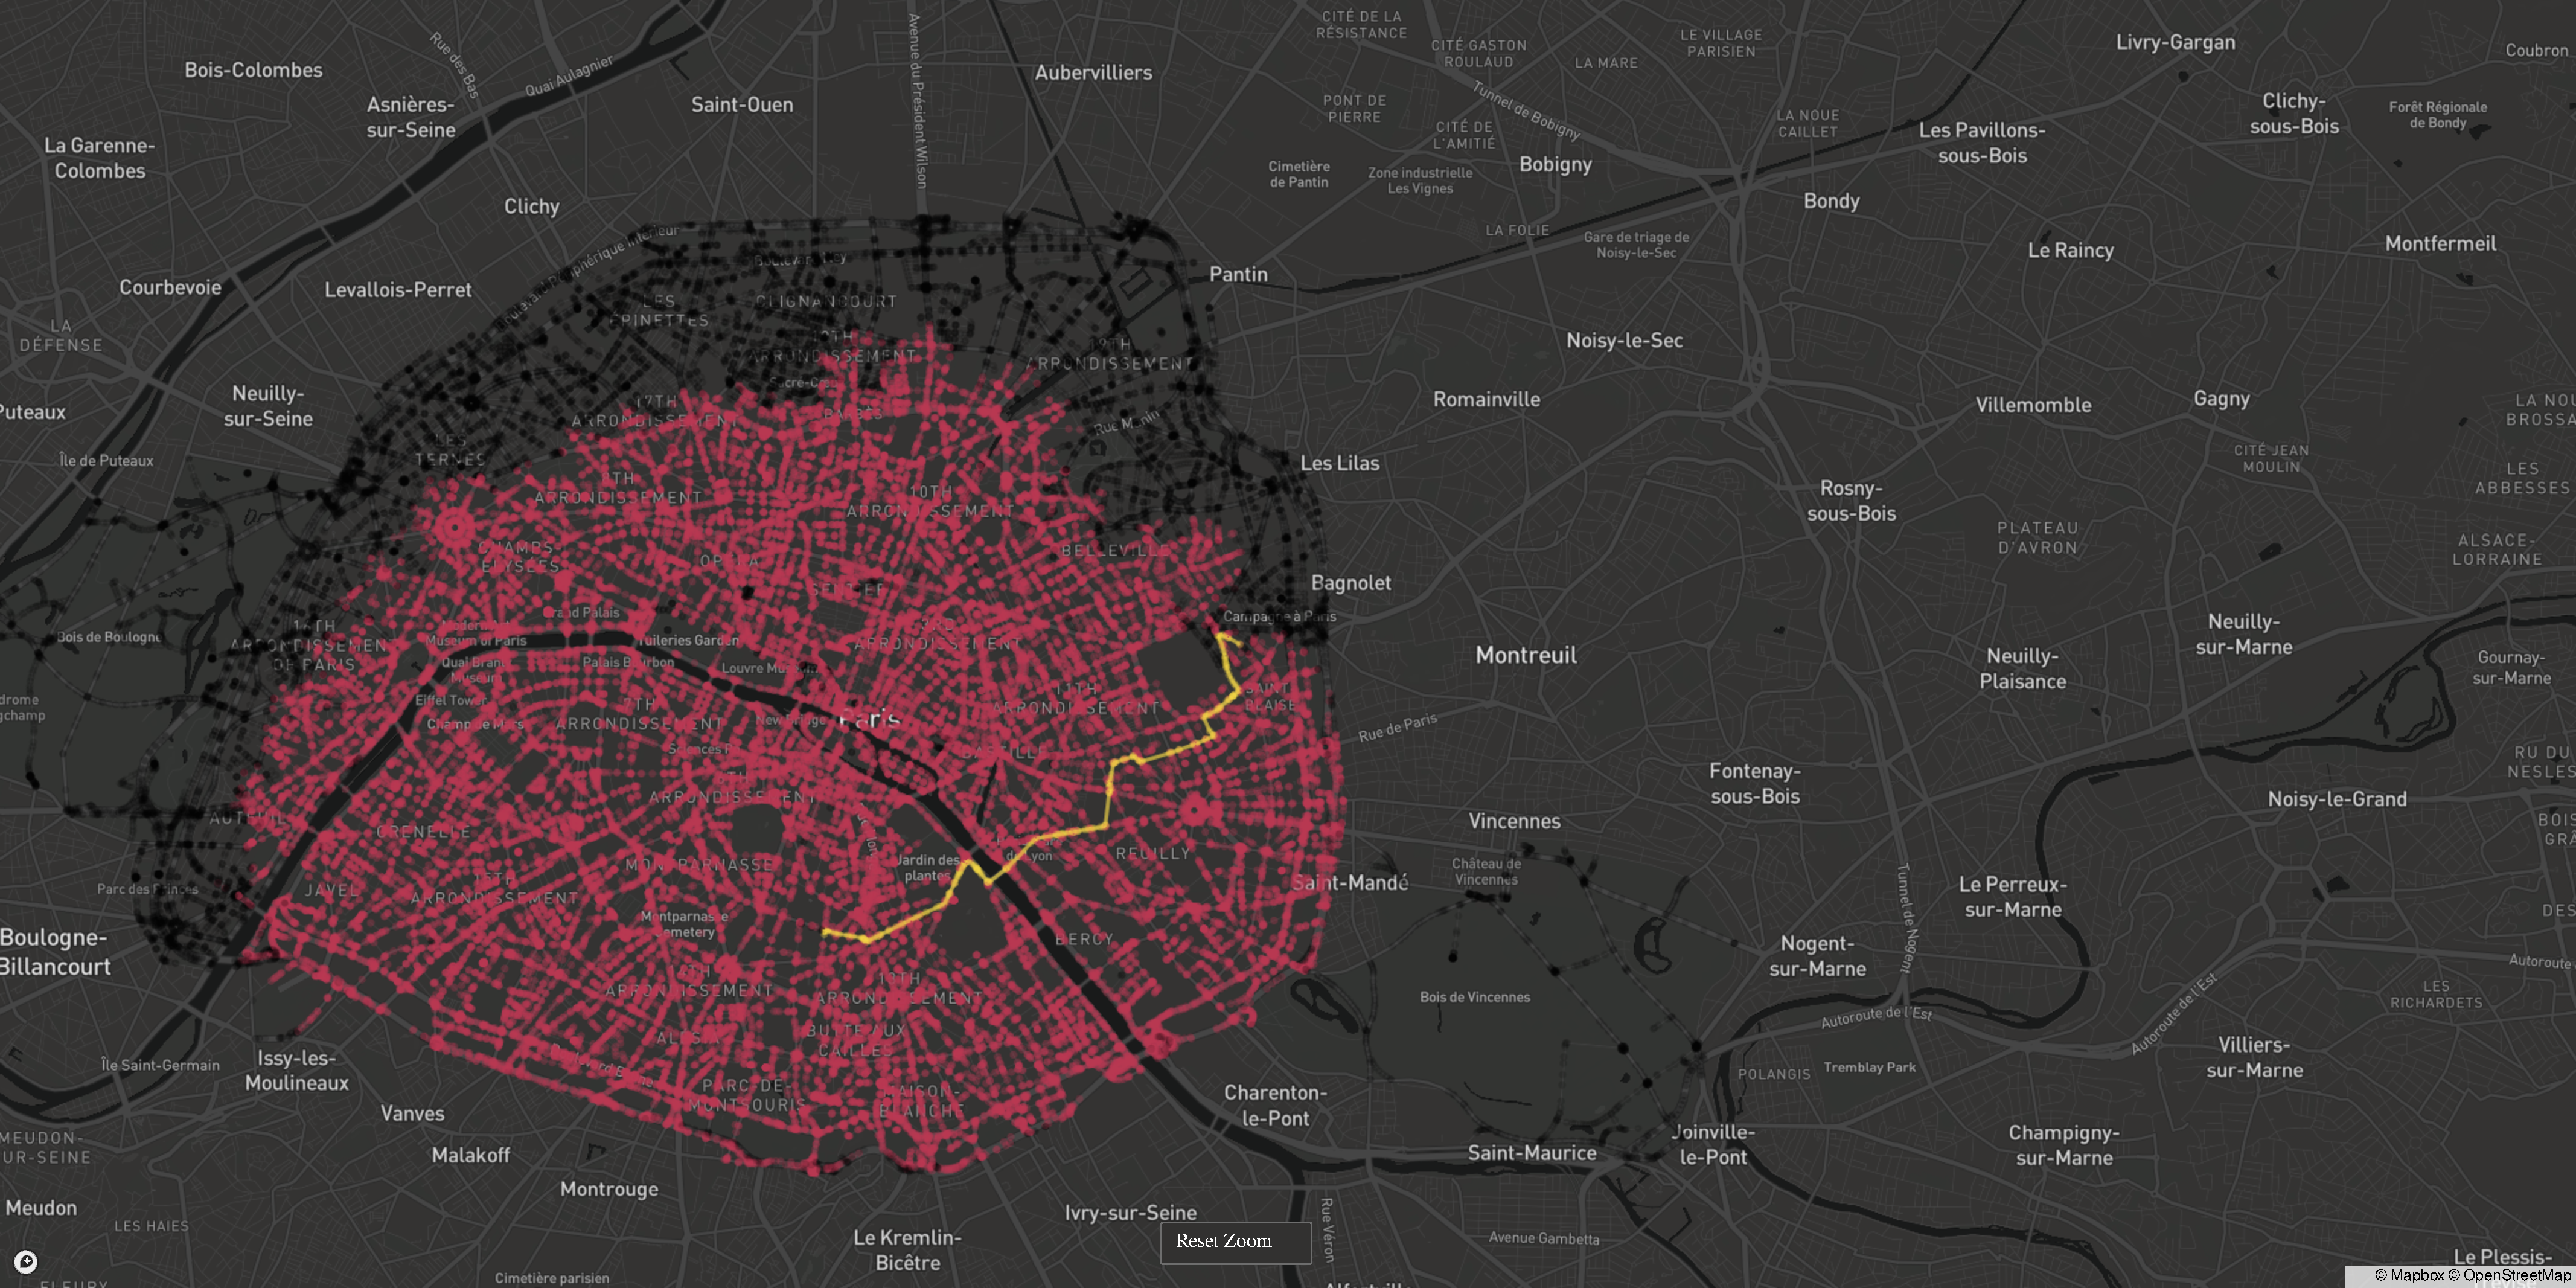
\includegraphics[height=0.9\textheight, keepaspectratio, trim={4cm 0 30cm 0}, clip ]{figures/paris_graph_based.pdf}
      \end{column}
  \end{columns}
\end{frame}

\begin{frame}[plain]{Node-based search (Baldur's Gate)}
  \begin{columns}[T]
      \begin{column}{.6\linewidth}
      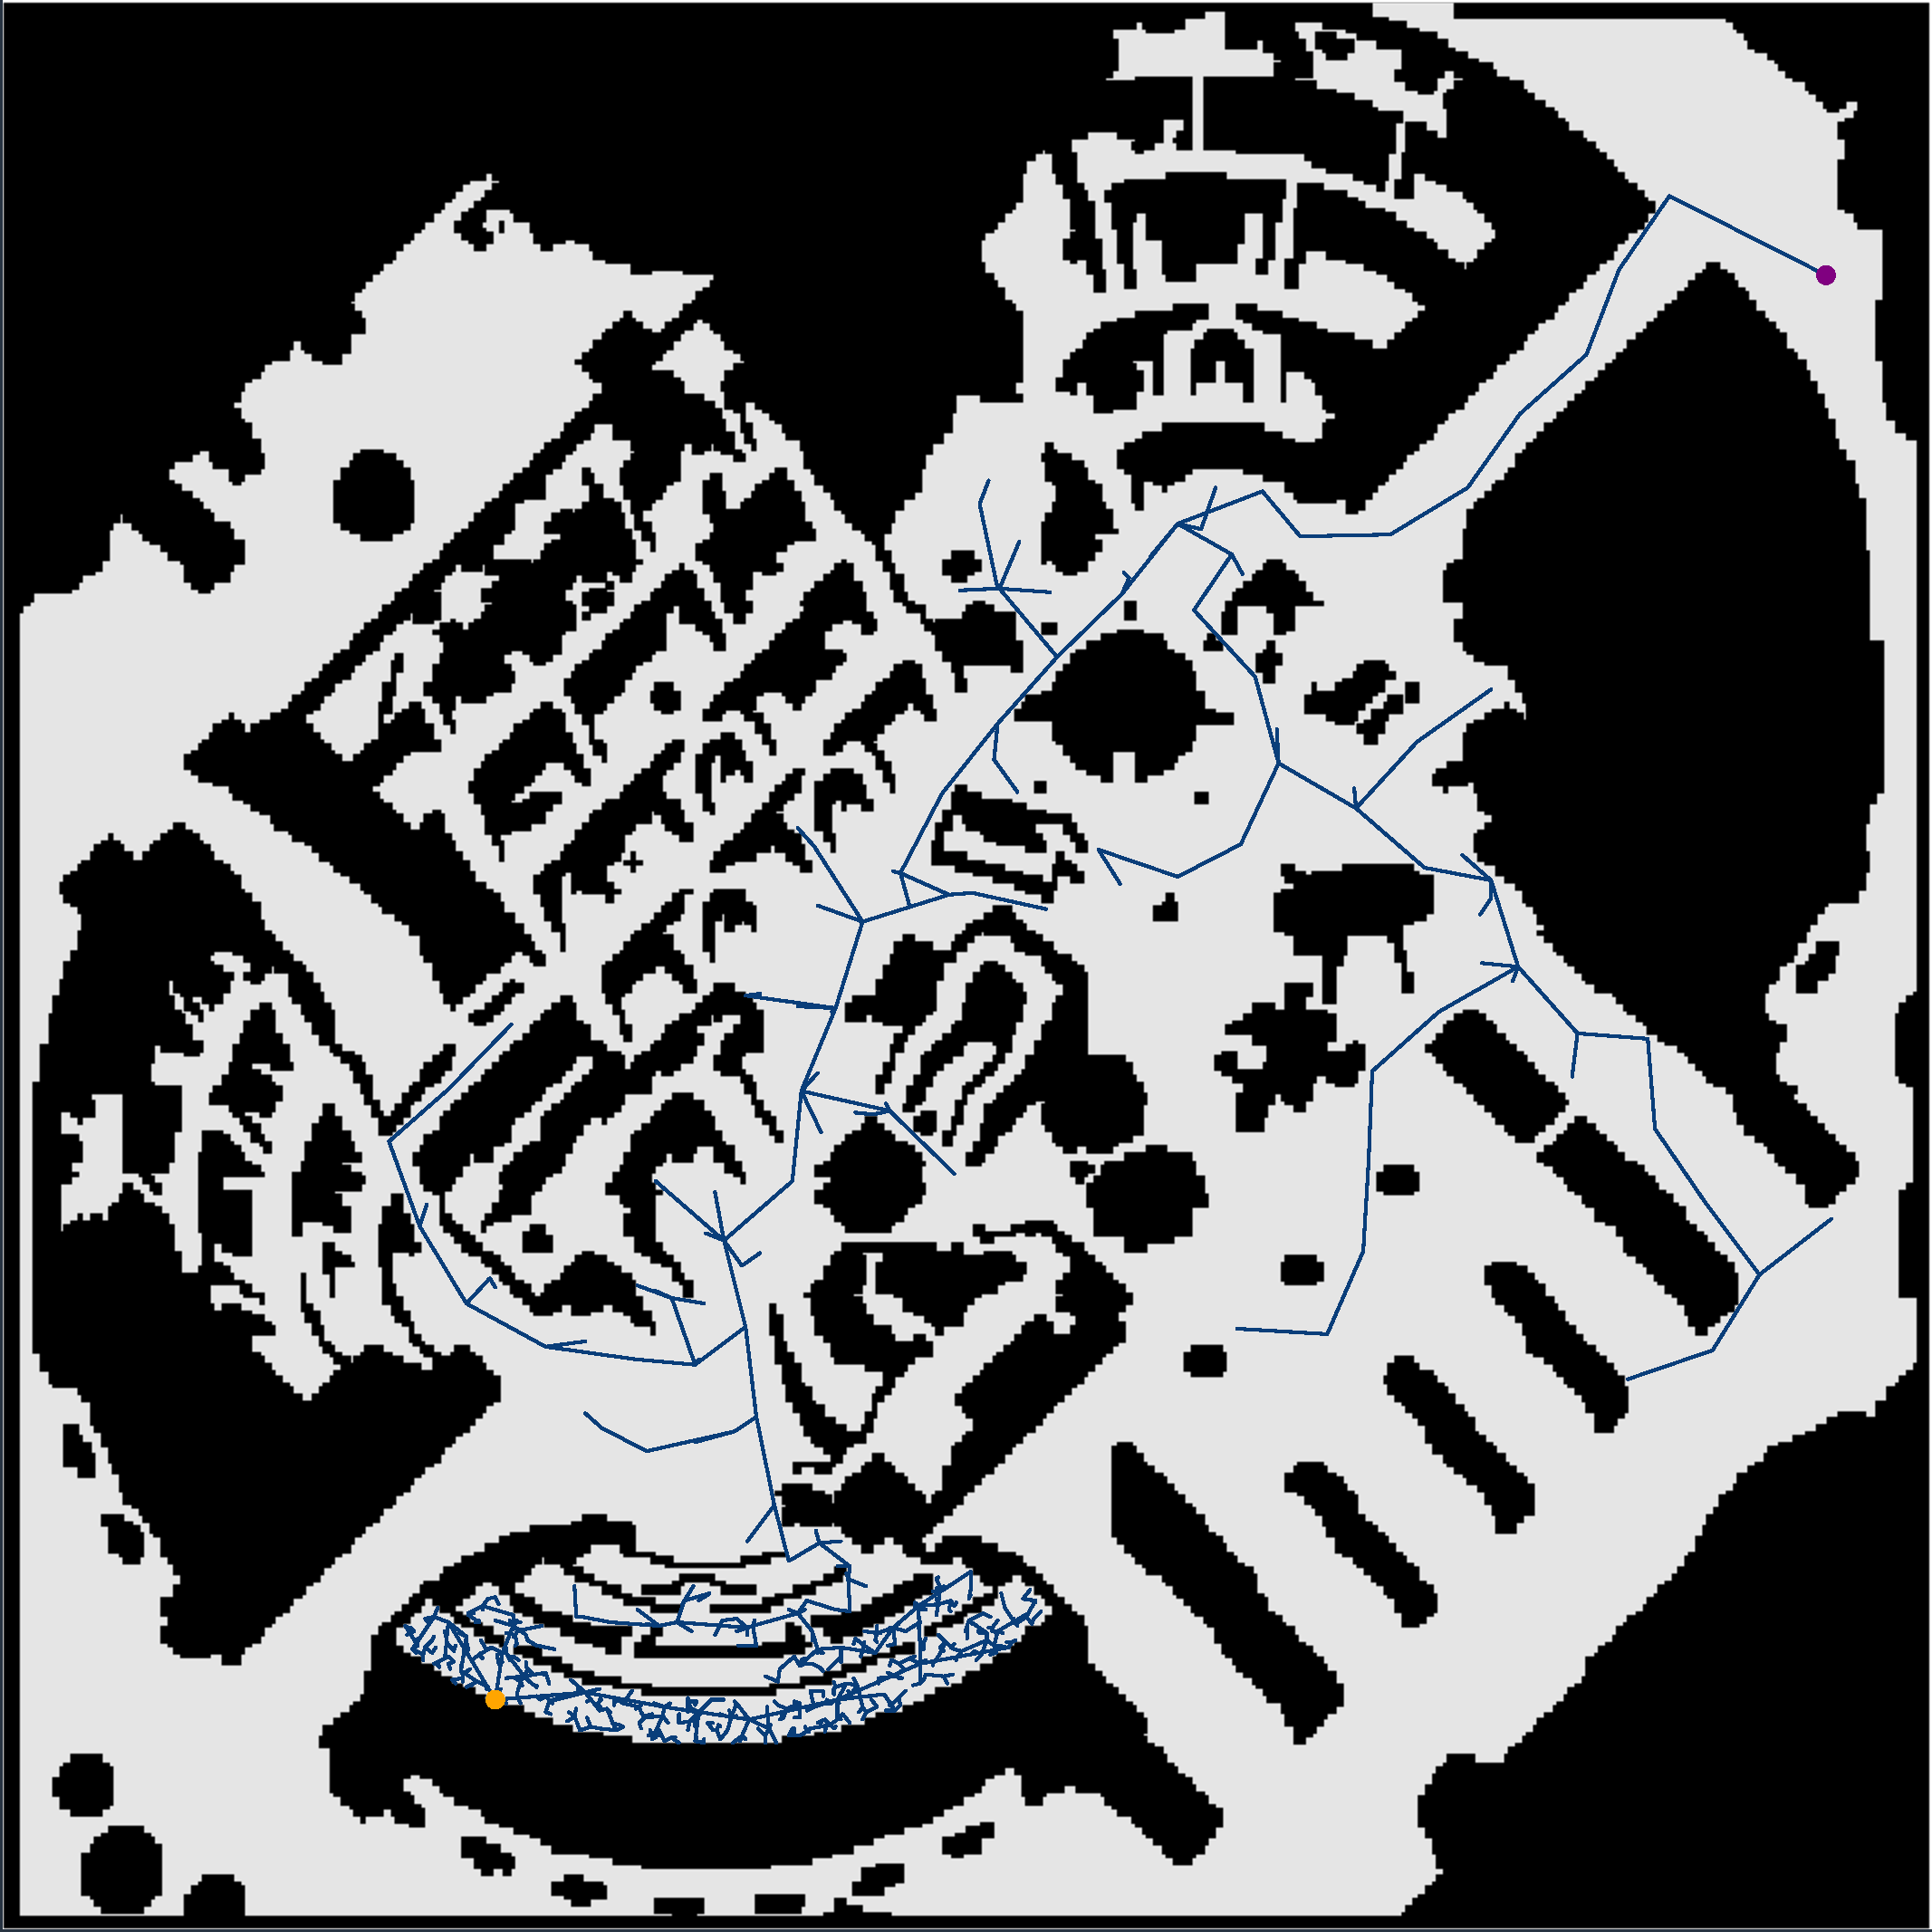
\includegraphics[height=0.9\textheight, keepaspectratio]{figures/baldurs_rrt_one_off.pdf}
      \end{column}
      \begin{column}{.4\linewidth}
          \begin{vfilleditems}
              \item {\Large Rapidly Exploring Random Trees}
              \item {\Large Probabilistic Roadmaps}
          \end{vfilleditems}
      \end{column}
  \end{columns}
\end{frame}

\begin{frame}{Maps {\Medium \color{white}( \cite{sturtevant2012benchmarks})}}
    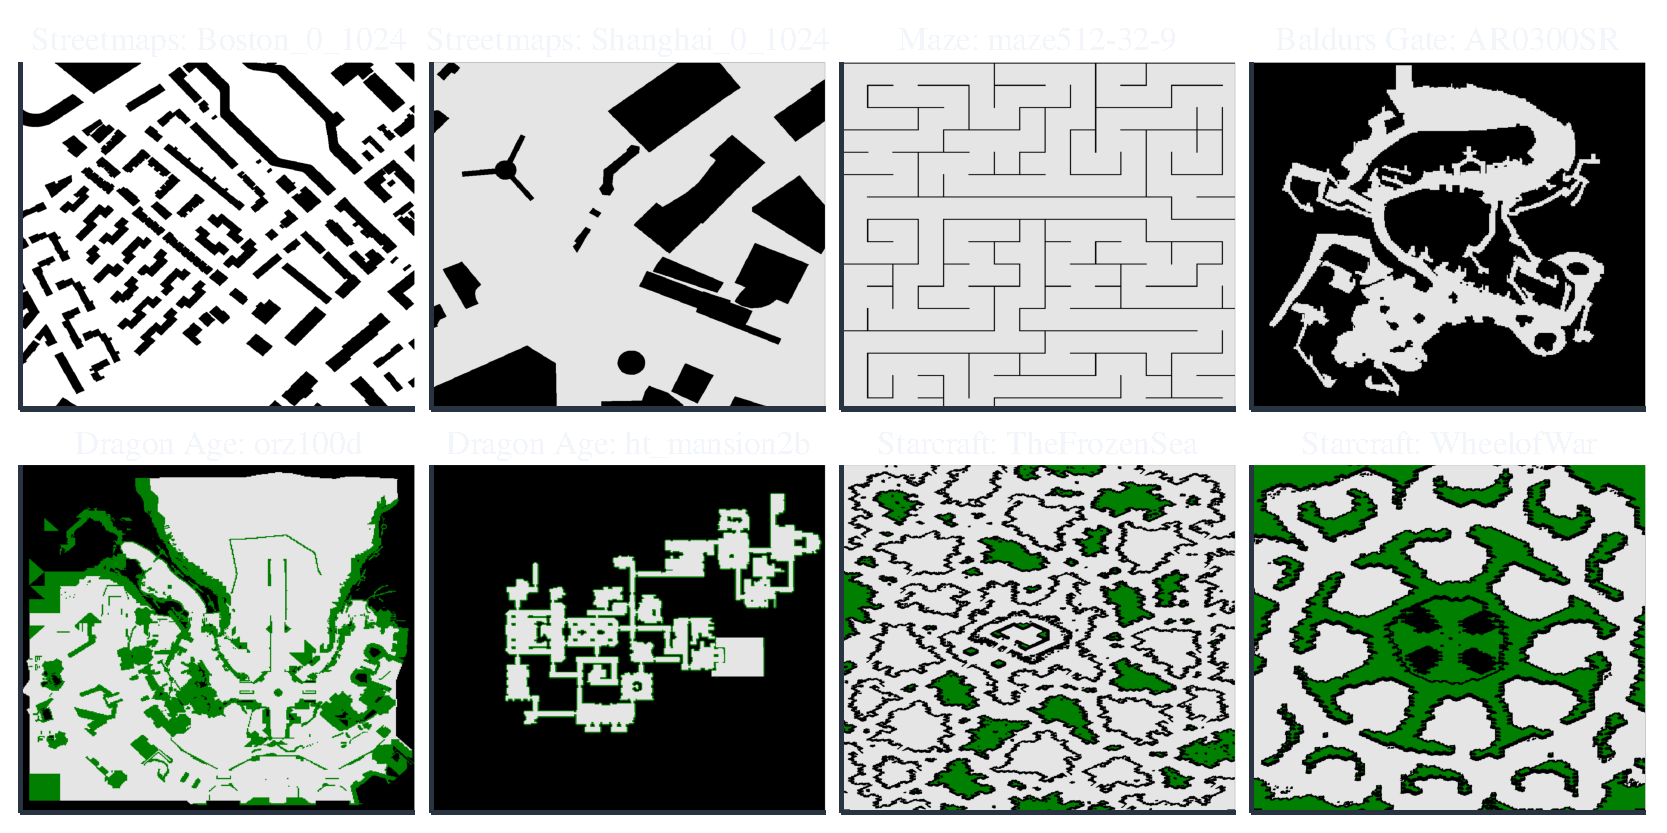
\includegraphics[width=1.0\linewidth, keepaspectratio]{figures/show_maps.pdf}
\end{frame}

\begin{frame}{Maps (Overview)}
    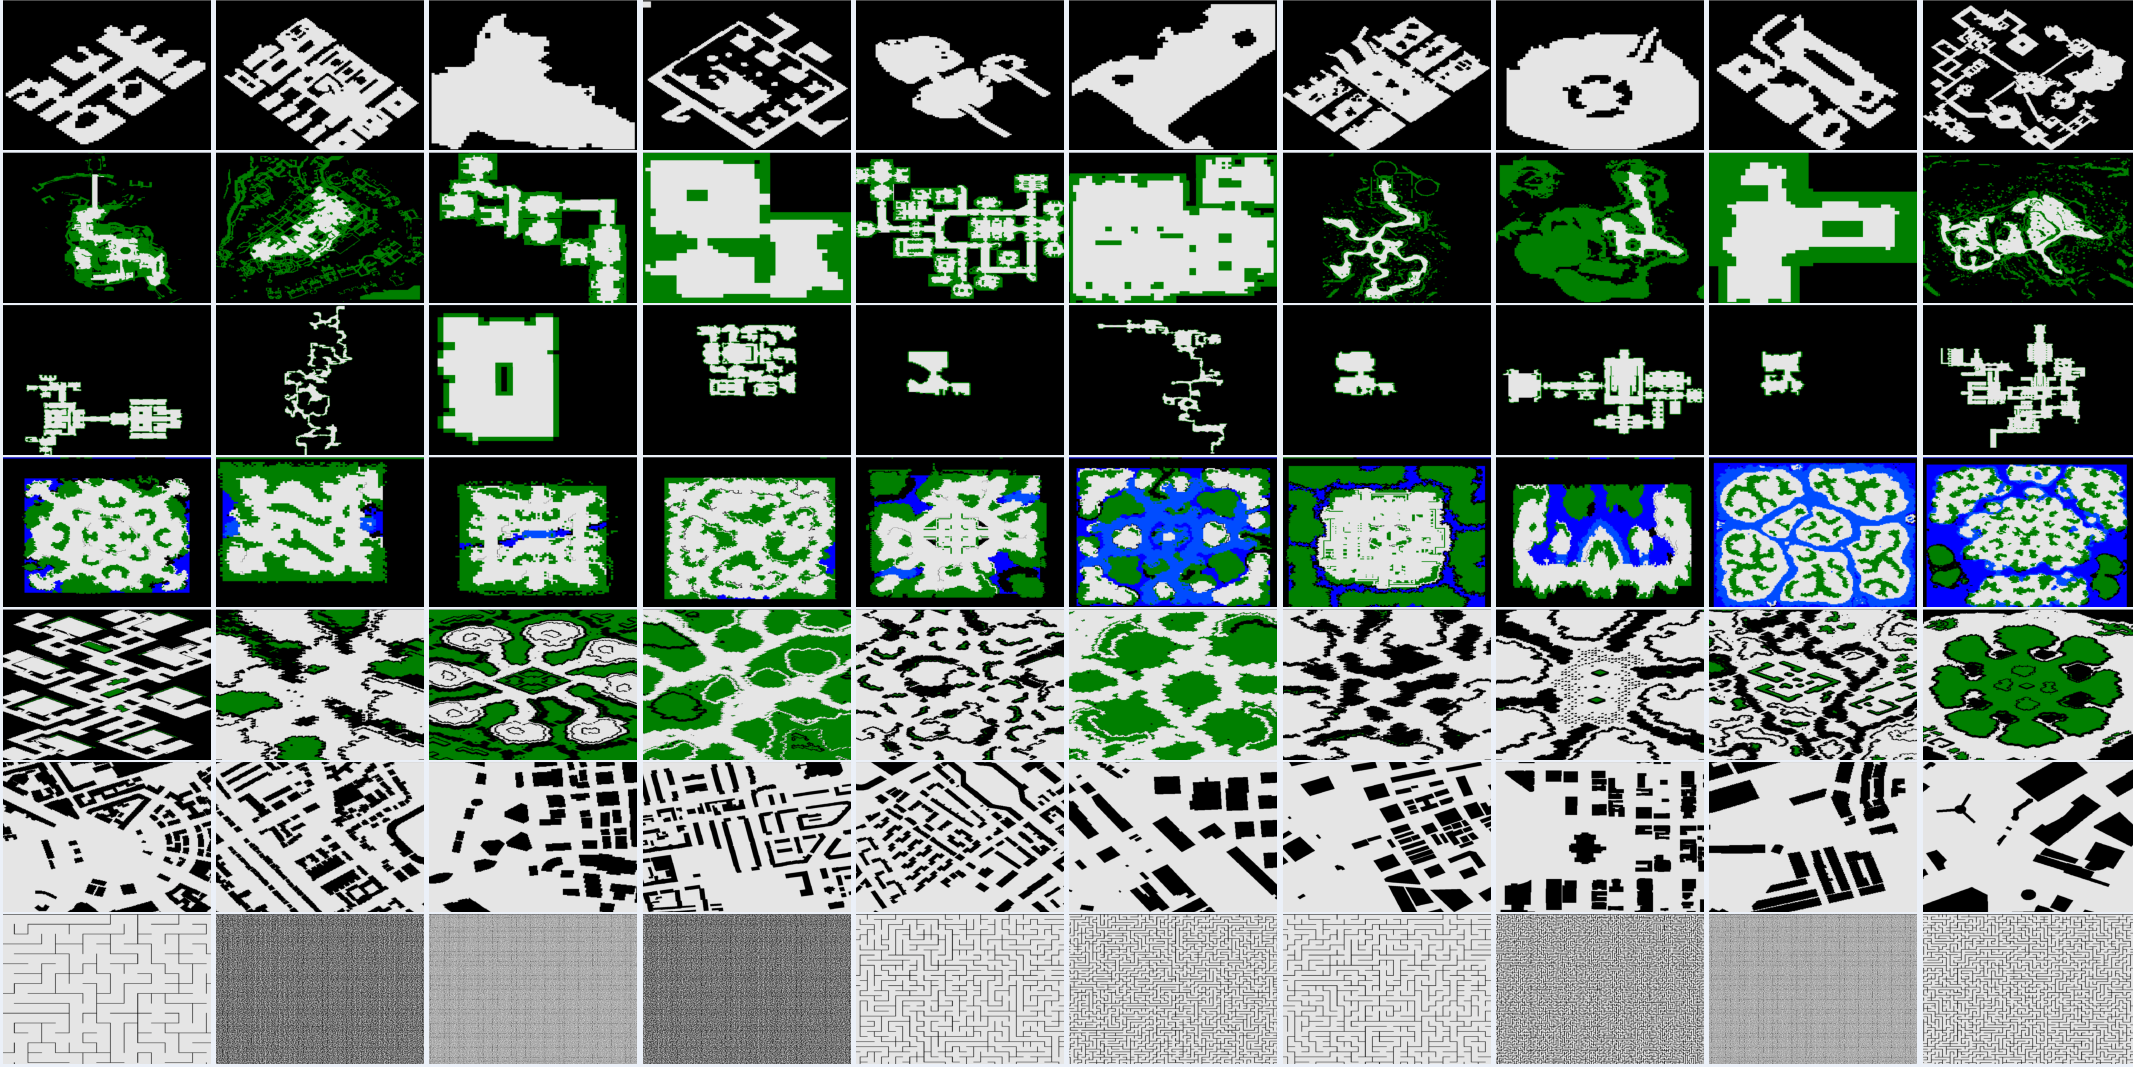
\includegraphics[width=1.0\linewidth, keepaspectratio]{figures/show_maps_overview.pdf}
\end{frame}

\begin{frame}{Outcomes}
    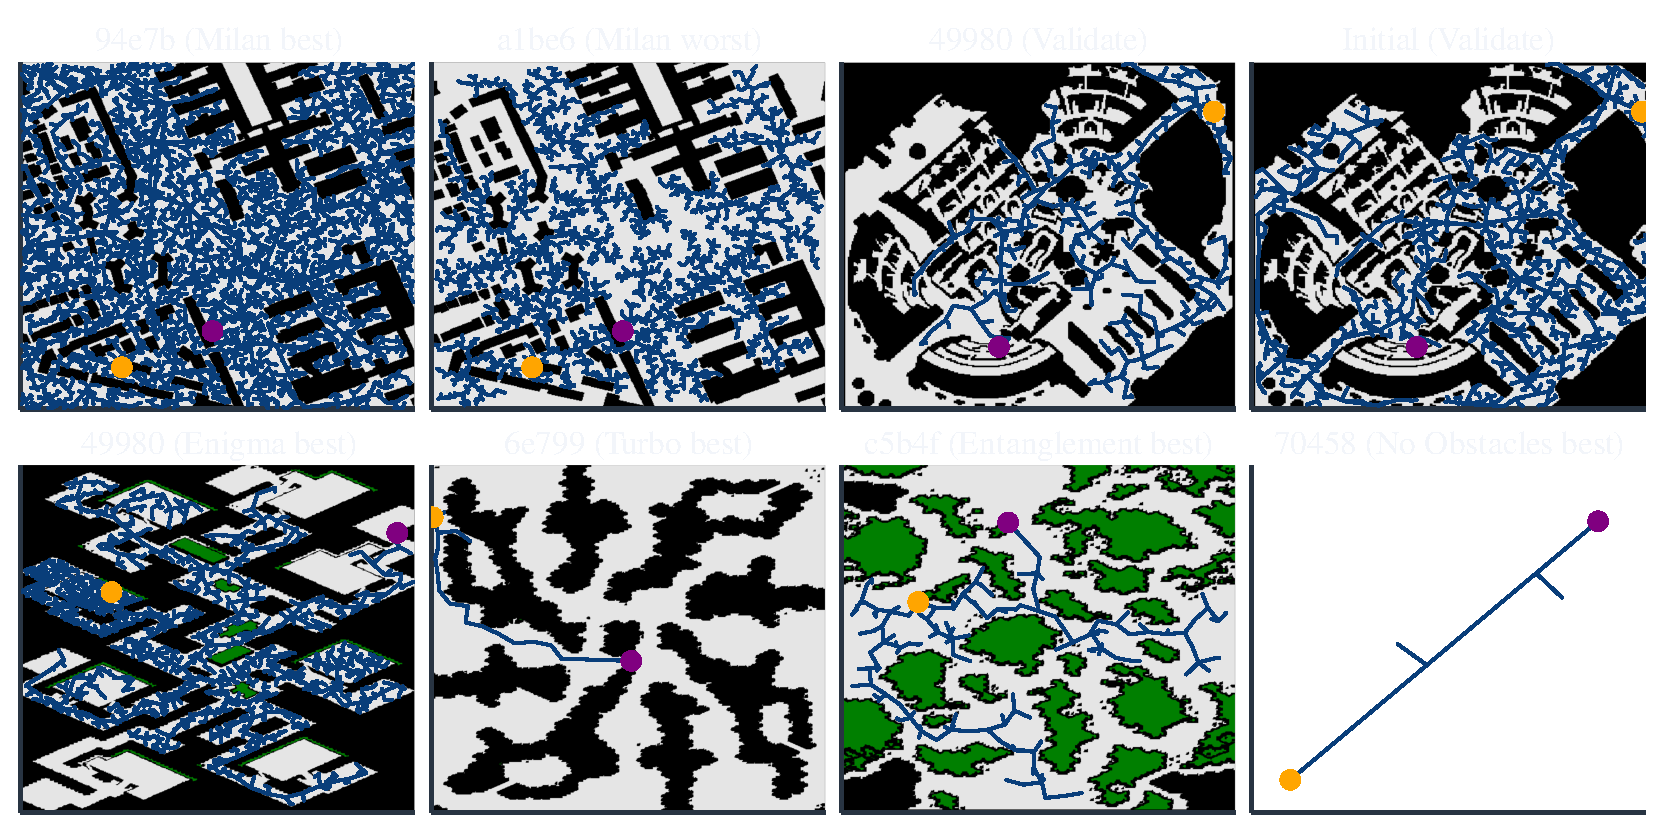
\includegraphics[width=1.0\linewidth, keepaspectratio]{figures/learned.pdf}
\end{frame}

\begin{frame}{{\color{pureminimalistic@text@white} Multiple Objectives}}
  \begin{columns}[T]
      \begin{column}{.4\linewidth}
          \begin{vfilleditems}
              \item \emph{Nodes}
              \item \emph{Path Length}
          \end{vfilleditems}
      \end{column}
      \begin{column}{.6\linewidth}
      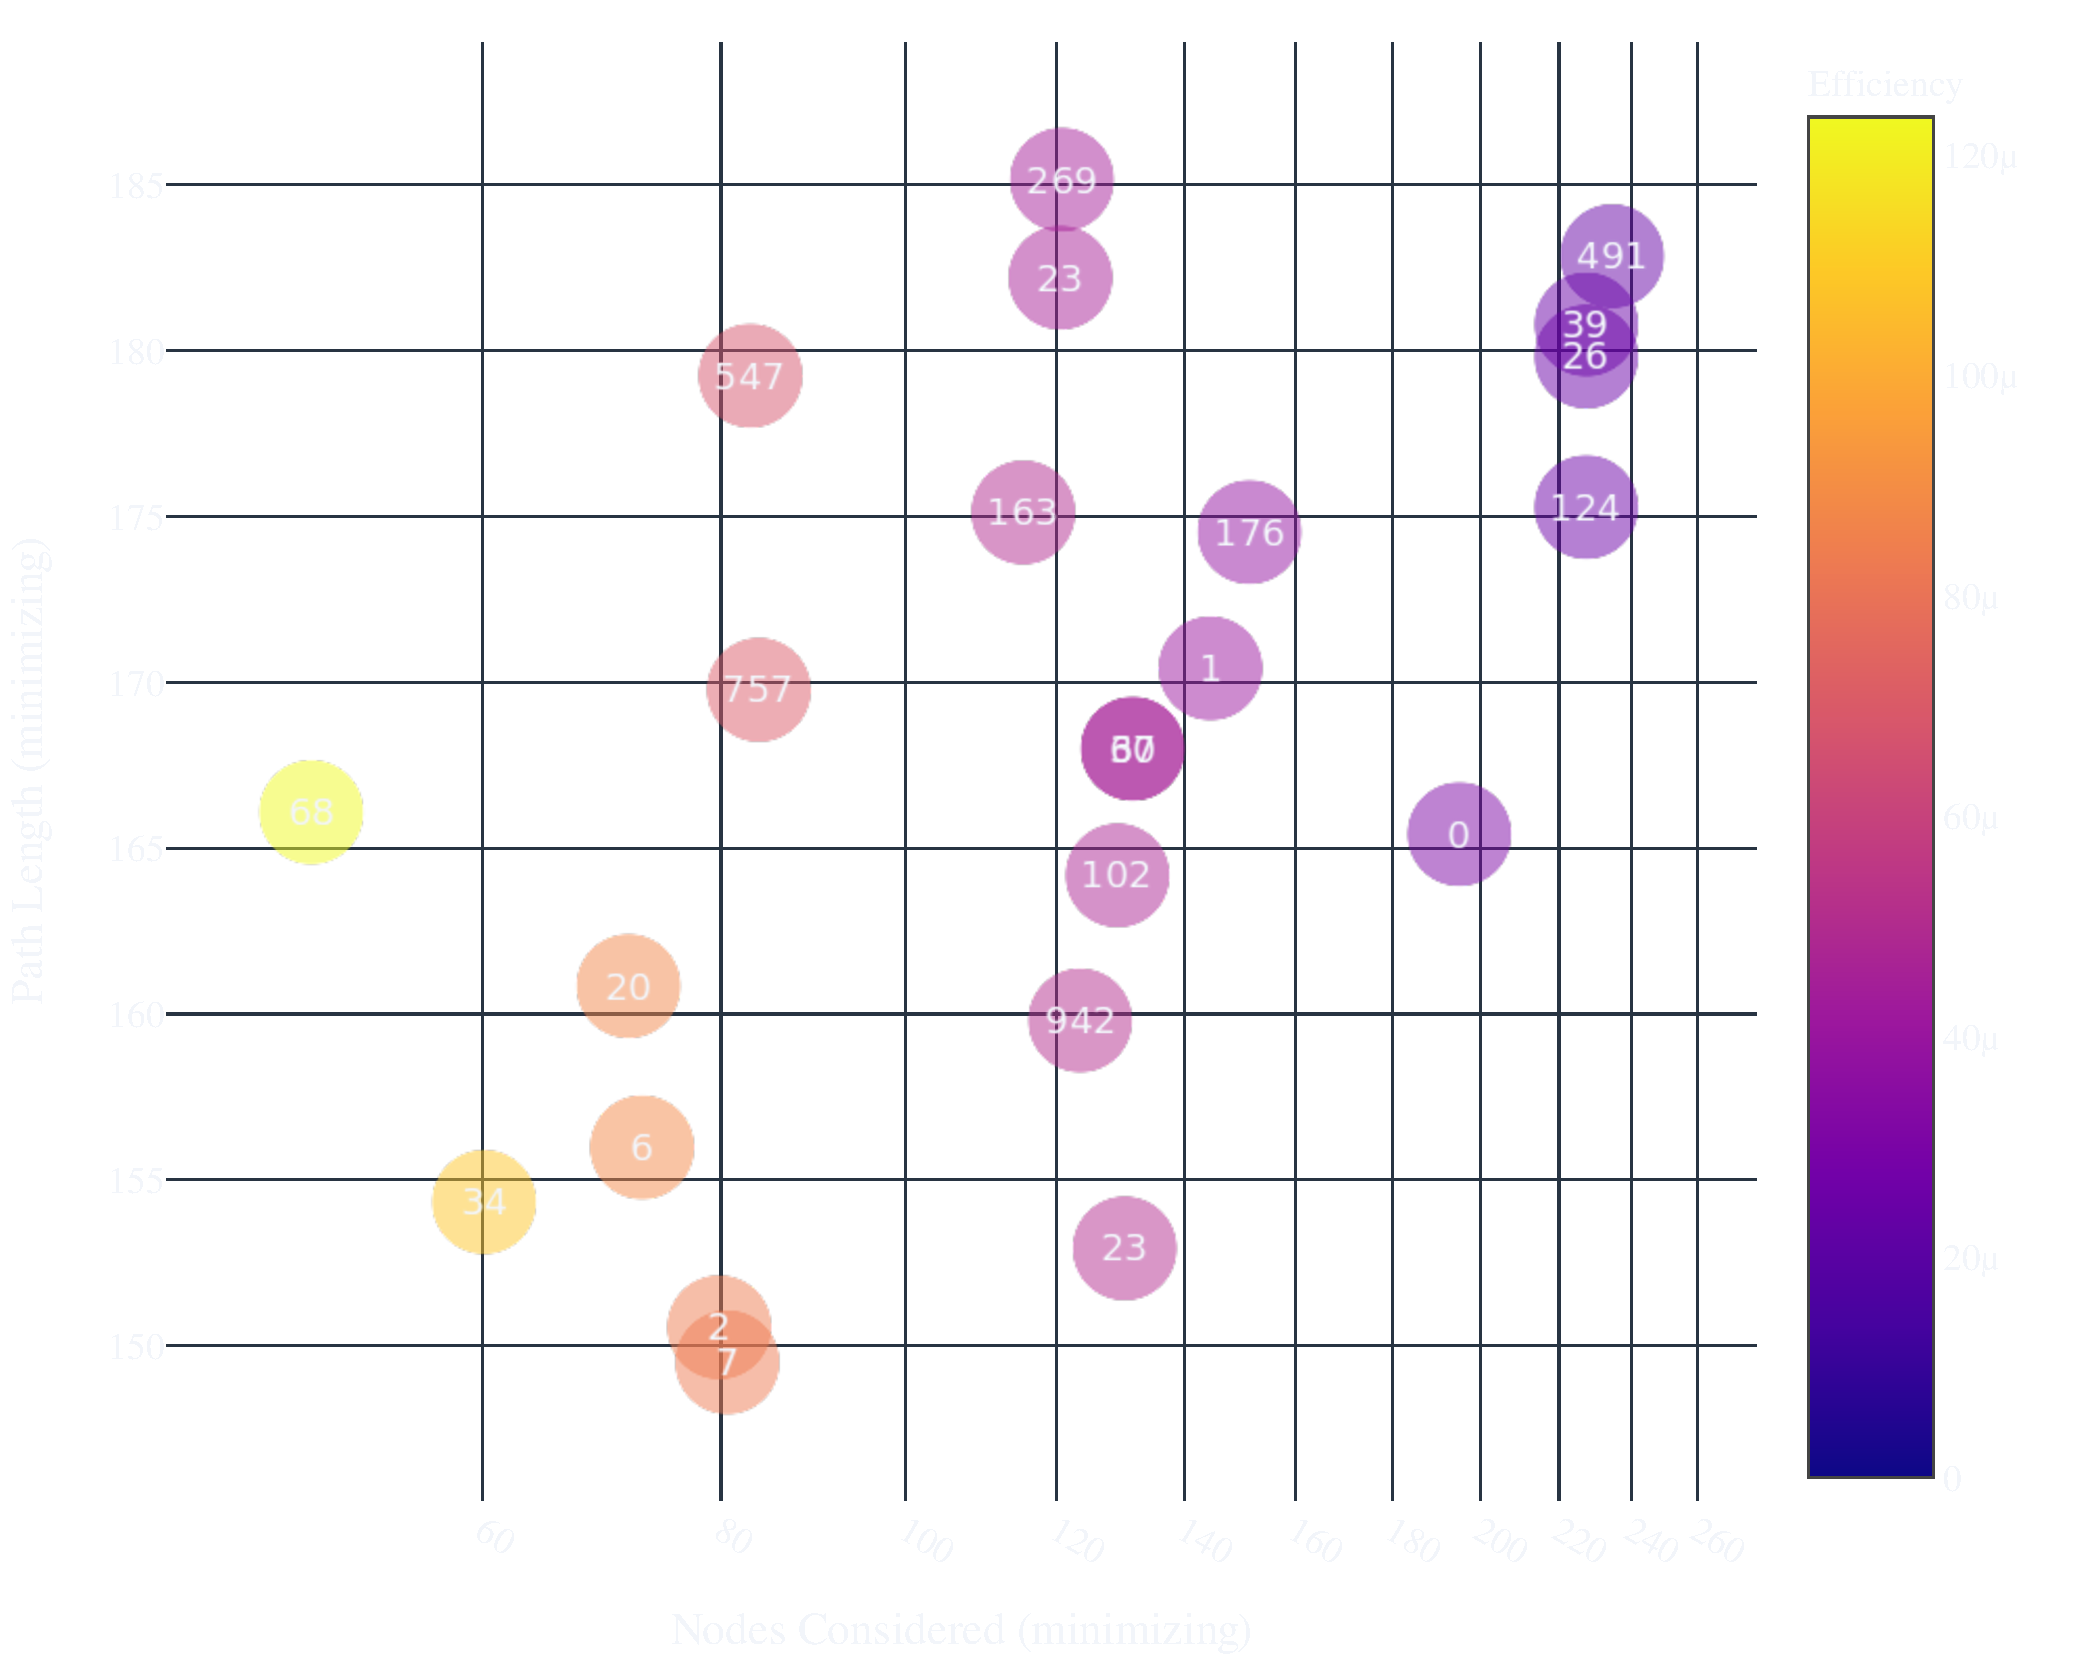
\includegraphics[width=0.9\linewidth, keepaspectratio]{figures/total_overview.pdf}
      \end{column}
  \end{columns}
\end{frame}

\begin{frame}{{Pareto Fronts}}
  \begin{columns}[T]
      \begin{column}{.4\linewidth}
          \begin{vfilleditems}
              \item {\Huge Trade-offs}
          \end{vfilleditems}
      \end{column}
      \begin{column}{.6\linewidth}
      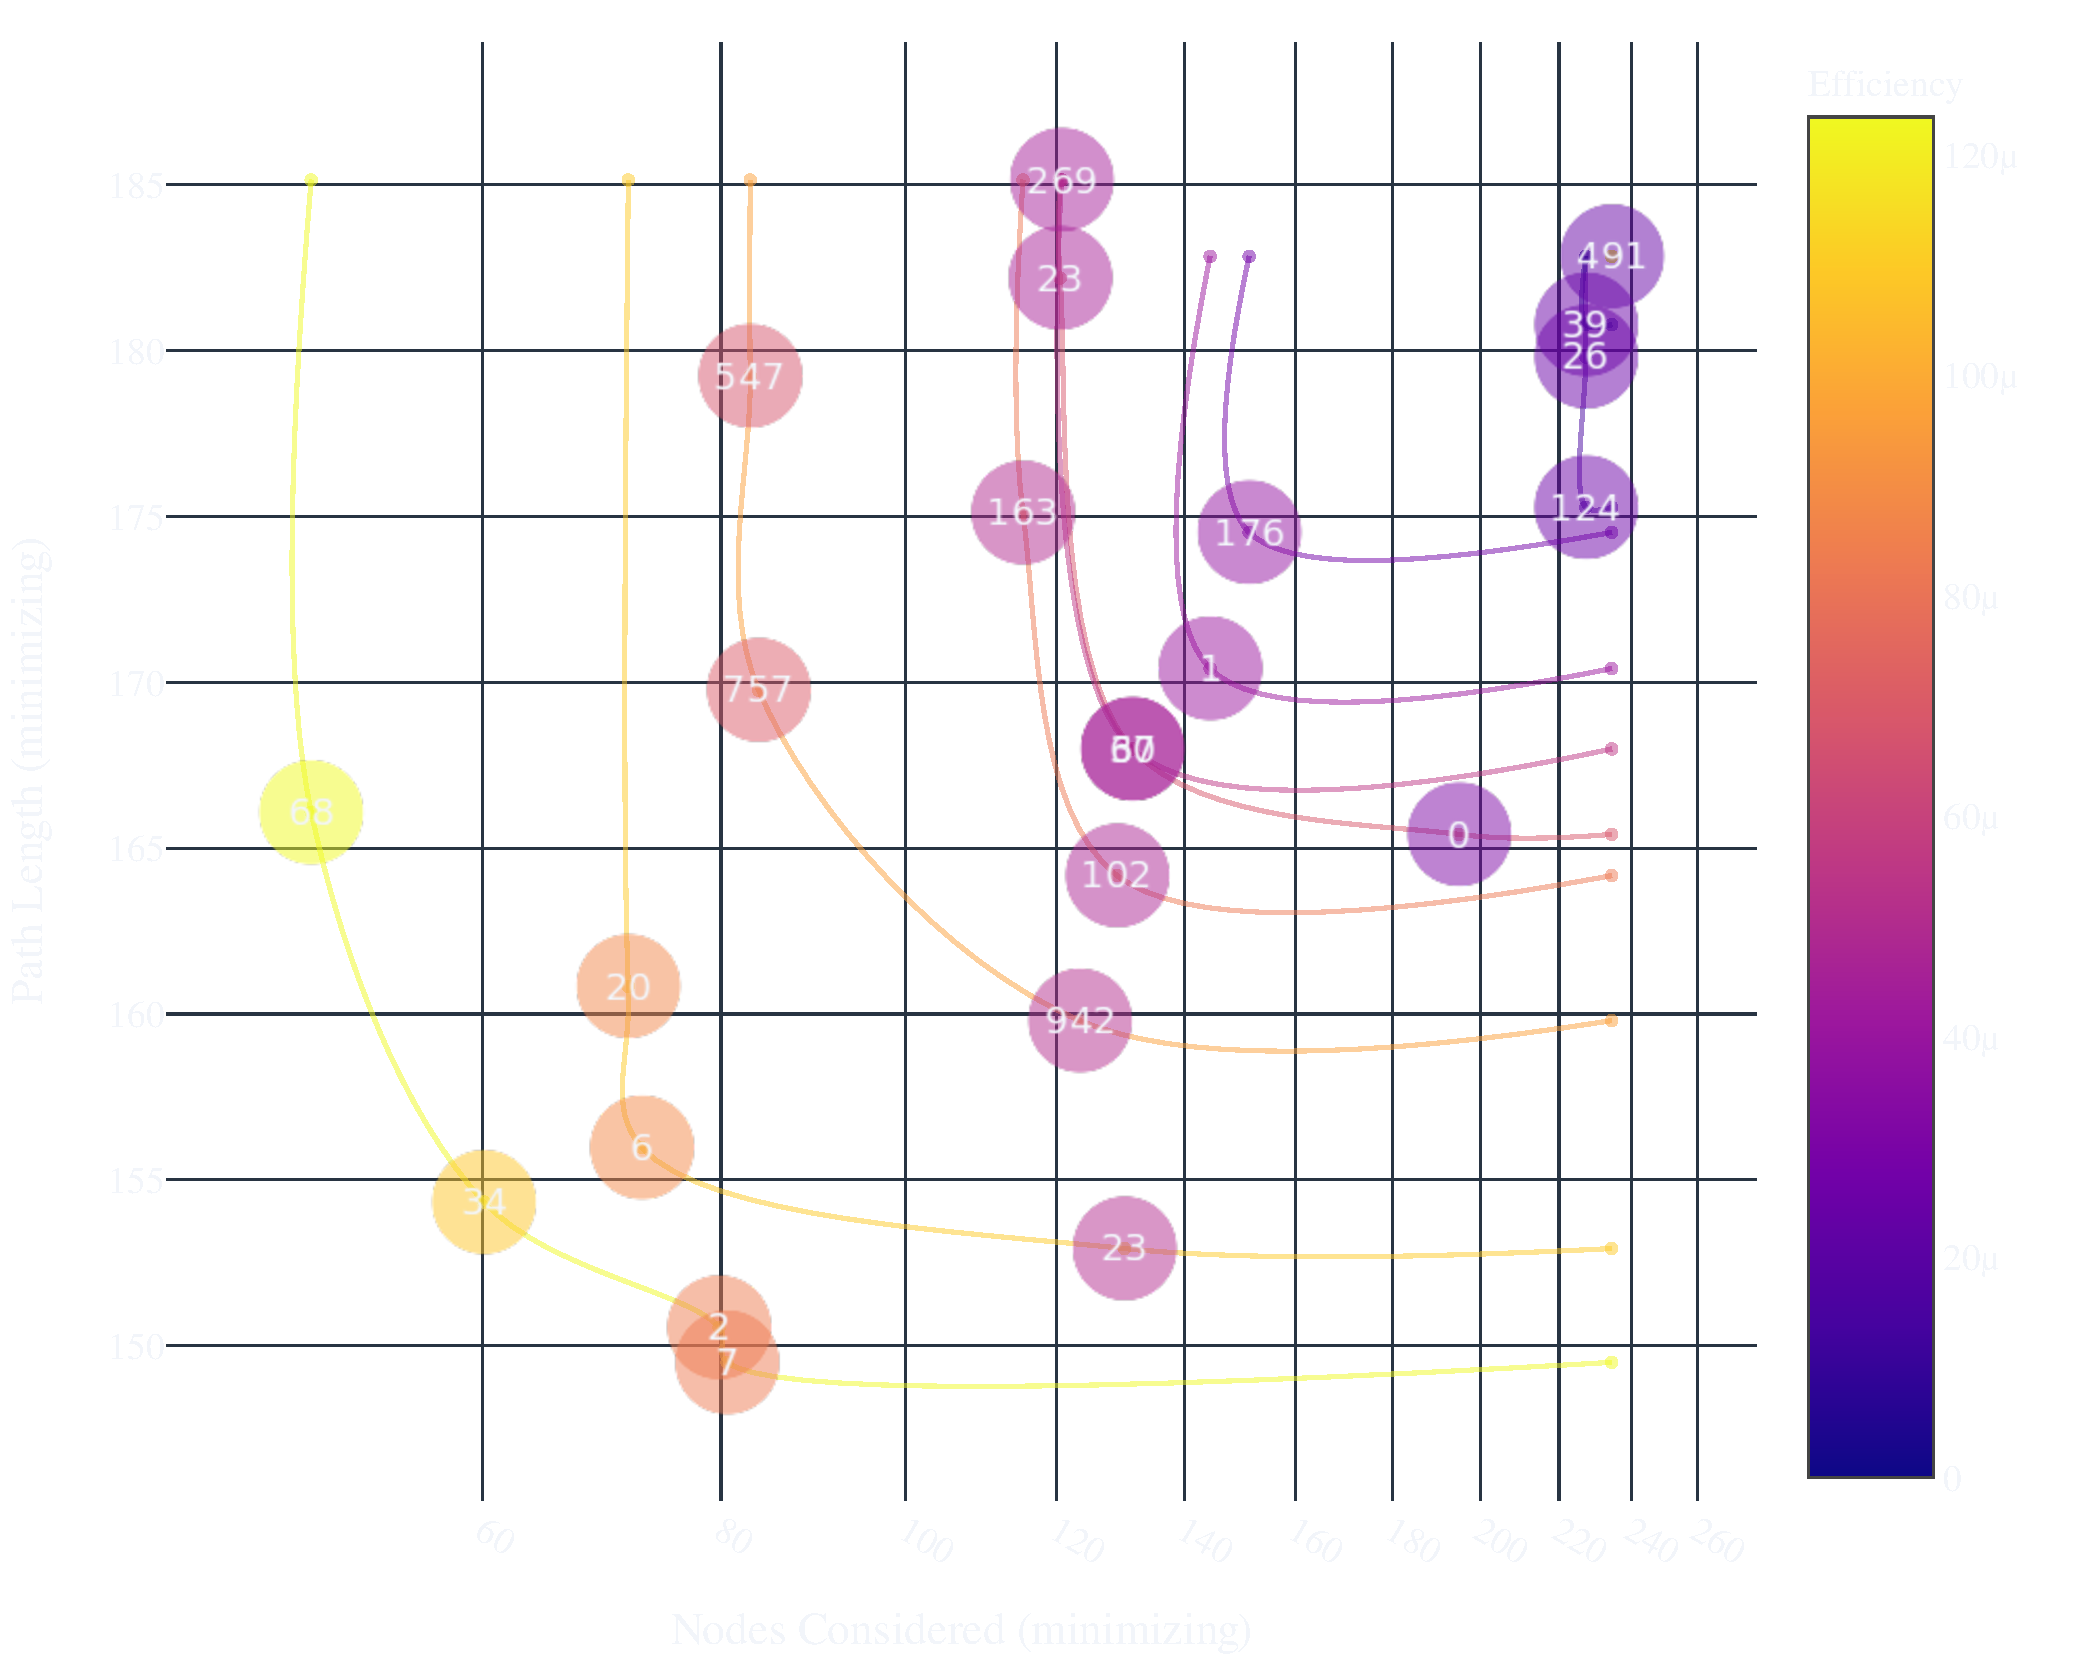
\includegraphics[width=0.9\linewidth, keepaspectratio]{figures/total_pareto_overview.pdf}
      \end{column}
  \end{columns}
\end{frame}

\begin{frame}{Pareto Evolution}
    \begin{vfilleditems}
        \item Why was it chosen?
        \item How does it work?
    \end{vfilleditems}
\end{frame}

\begin{frame}{Pareto Evolution}
    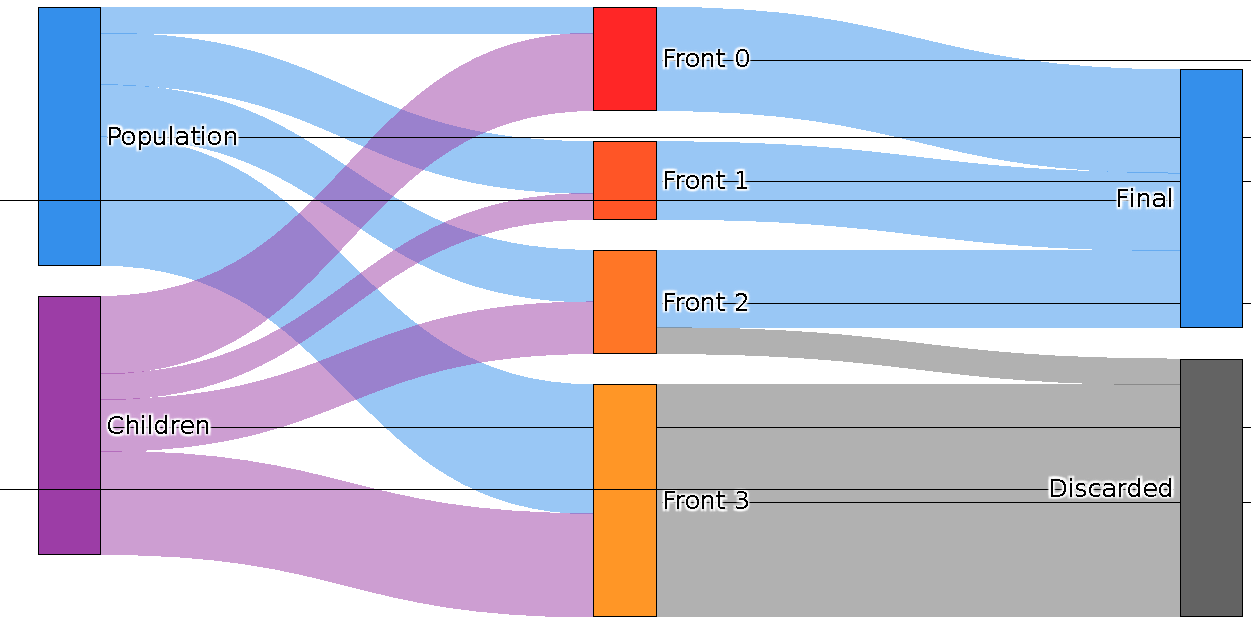
\includegraphics[width=1.0\linewidth, keepaspectratio]{figures/paretoev.pdf}
\end{frame}

\begin{frame}{Population Dynamics: Starcraft Engima}
    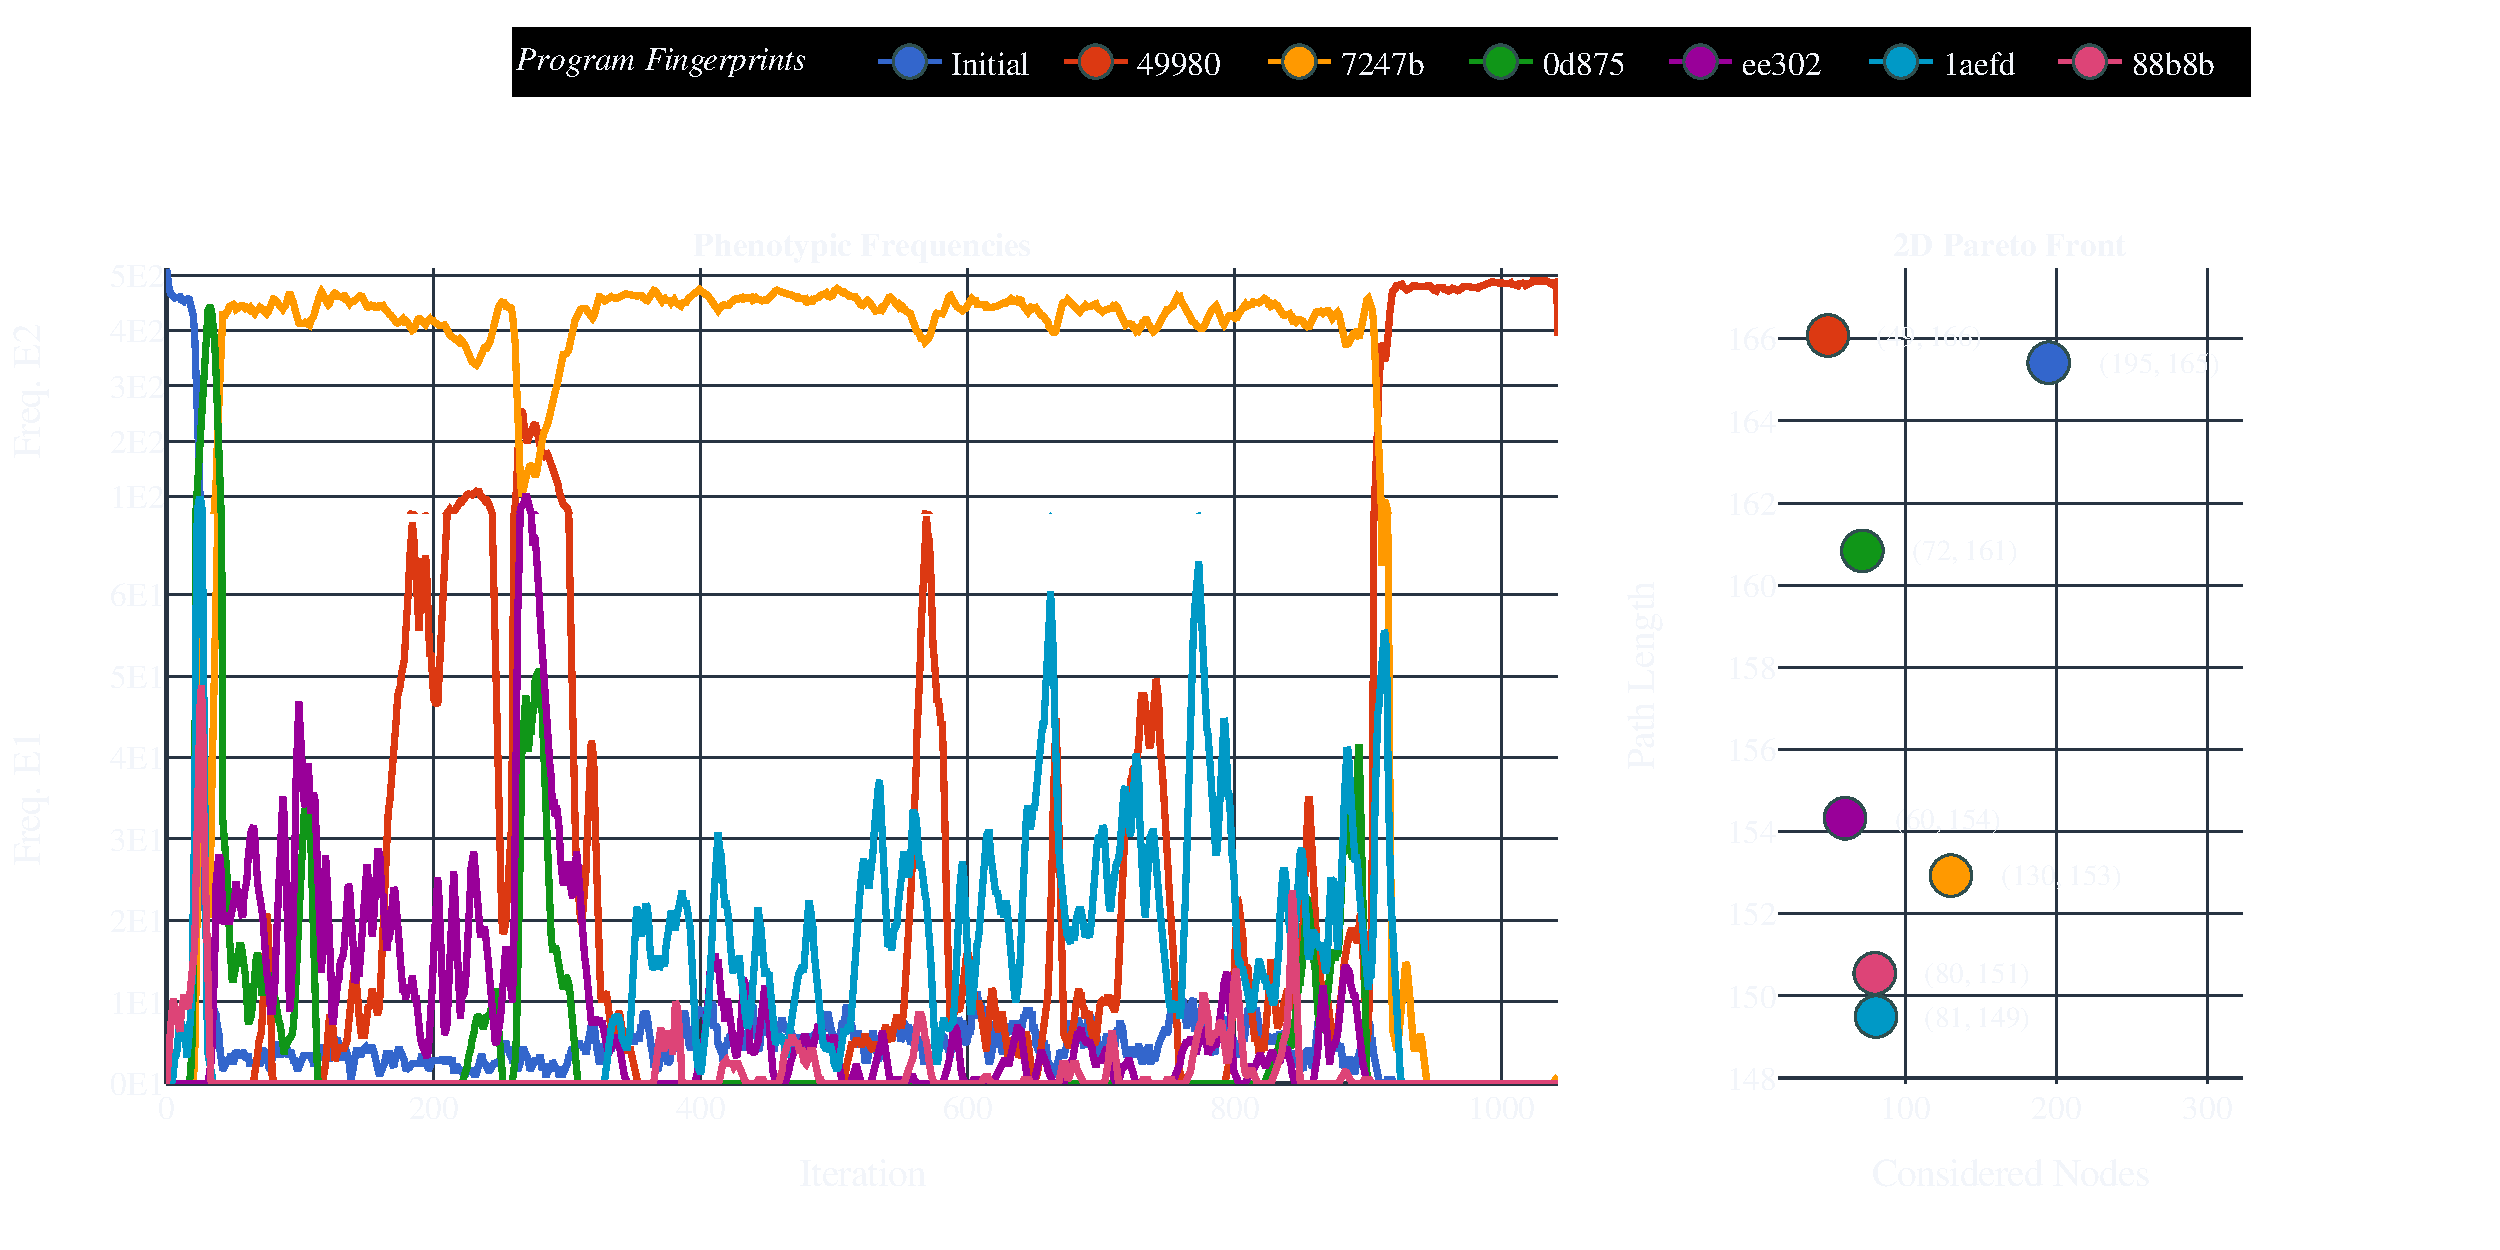
\includegraphics[width=1.0\linewidth, keepaspectratio]{figures/pheno.pdf}
\end{frame}

\begin{frame}{Population Dynamics: Baldur's Gate}
    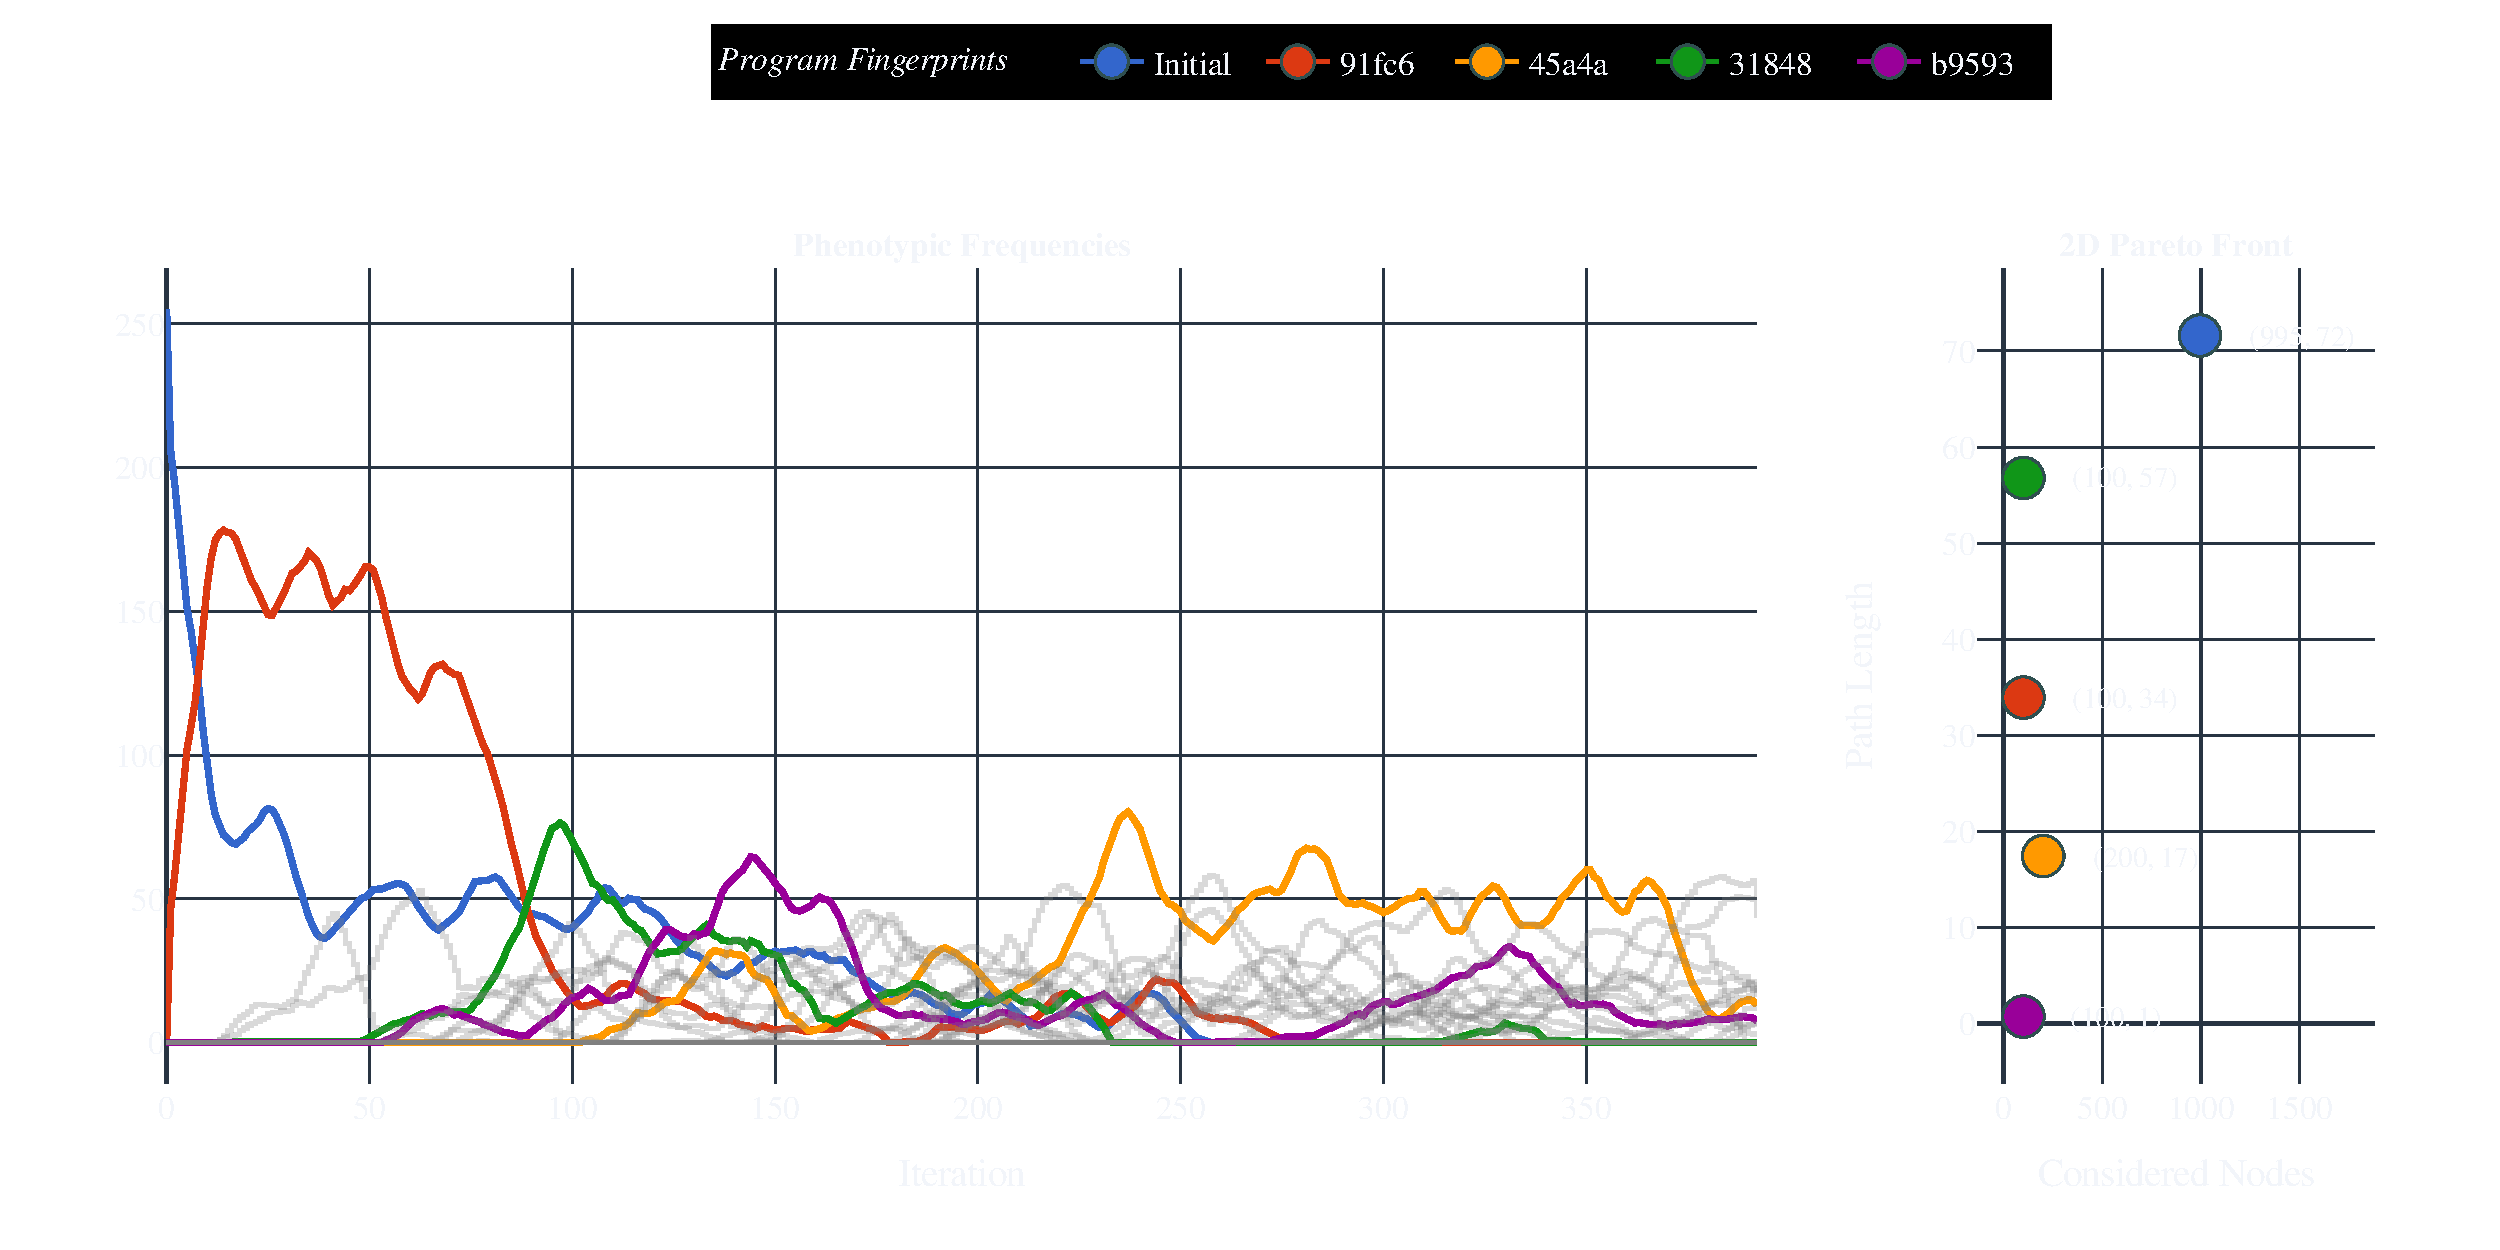
\includegraphics[width=1.0\linewidth, keepaspectratio]{figures/baldurs_pheno_60.pdf}
\end{frame}

\appendix % do not count the following slides for the total number
\section*{Backup Slides}
\begin{frame}[plain, noframenumbering]
  \centering
  \vfill
  {\fontsize{40}{50}\selectfont Questions?}
  \vfill
\end{frame}

\begin{frame}[plain, noframenumbering]
  \centering
  \printbibliography
\end{frame}

\begin{frame}[plain]{Thesis}
    \begin{vfilleditems}
      \item {\Huge Evolution is powerful}
        \begin{itemize}
          \item {\Medium Responsible for Earth's diverse, adaptive life}
          \item {\Medium \color{pureminimalistic@text@red} Evolved intelligence}
        \end{itemize}
      \item {\Huge Learned representation matters}
    \end{vfilleditems}
\end{frame}

\begin{frame}{Research Questions}
  \begin{vfilleditems}
    \item {\Huge Is Genetic Programming Competitive in 2021? {\color{pureminimalistic@text@red} Yes.}}
    % TODO: Answer each at high level
    {\color{grey}
    \item {\Huge Is crossover necessary?}
    \item {\Huge What is the role of latent code?}
    \item {\Huge How should code be mutated?}
    \item {\Huge How hard is a problem?}
    }
  \end{vfilleditems}
\end{frame}

\begin{frame}{Research Questions}
  \begin{vfilleditems}
    \item {\Huge Role of program representation?}
    \item {\Huge Role of scale and compute efficiency?}
    \item {\Huge How should code be mutated?}
    \item {\Huge How hard is a problem?}
  \end{vfilleditems}
\end{frame}

\begin{frame}{Population Dynamics: Baldur's Gate}
    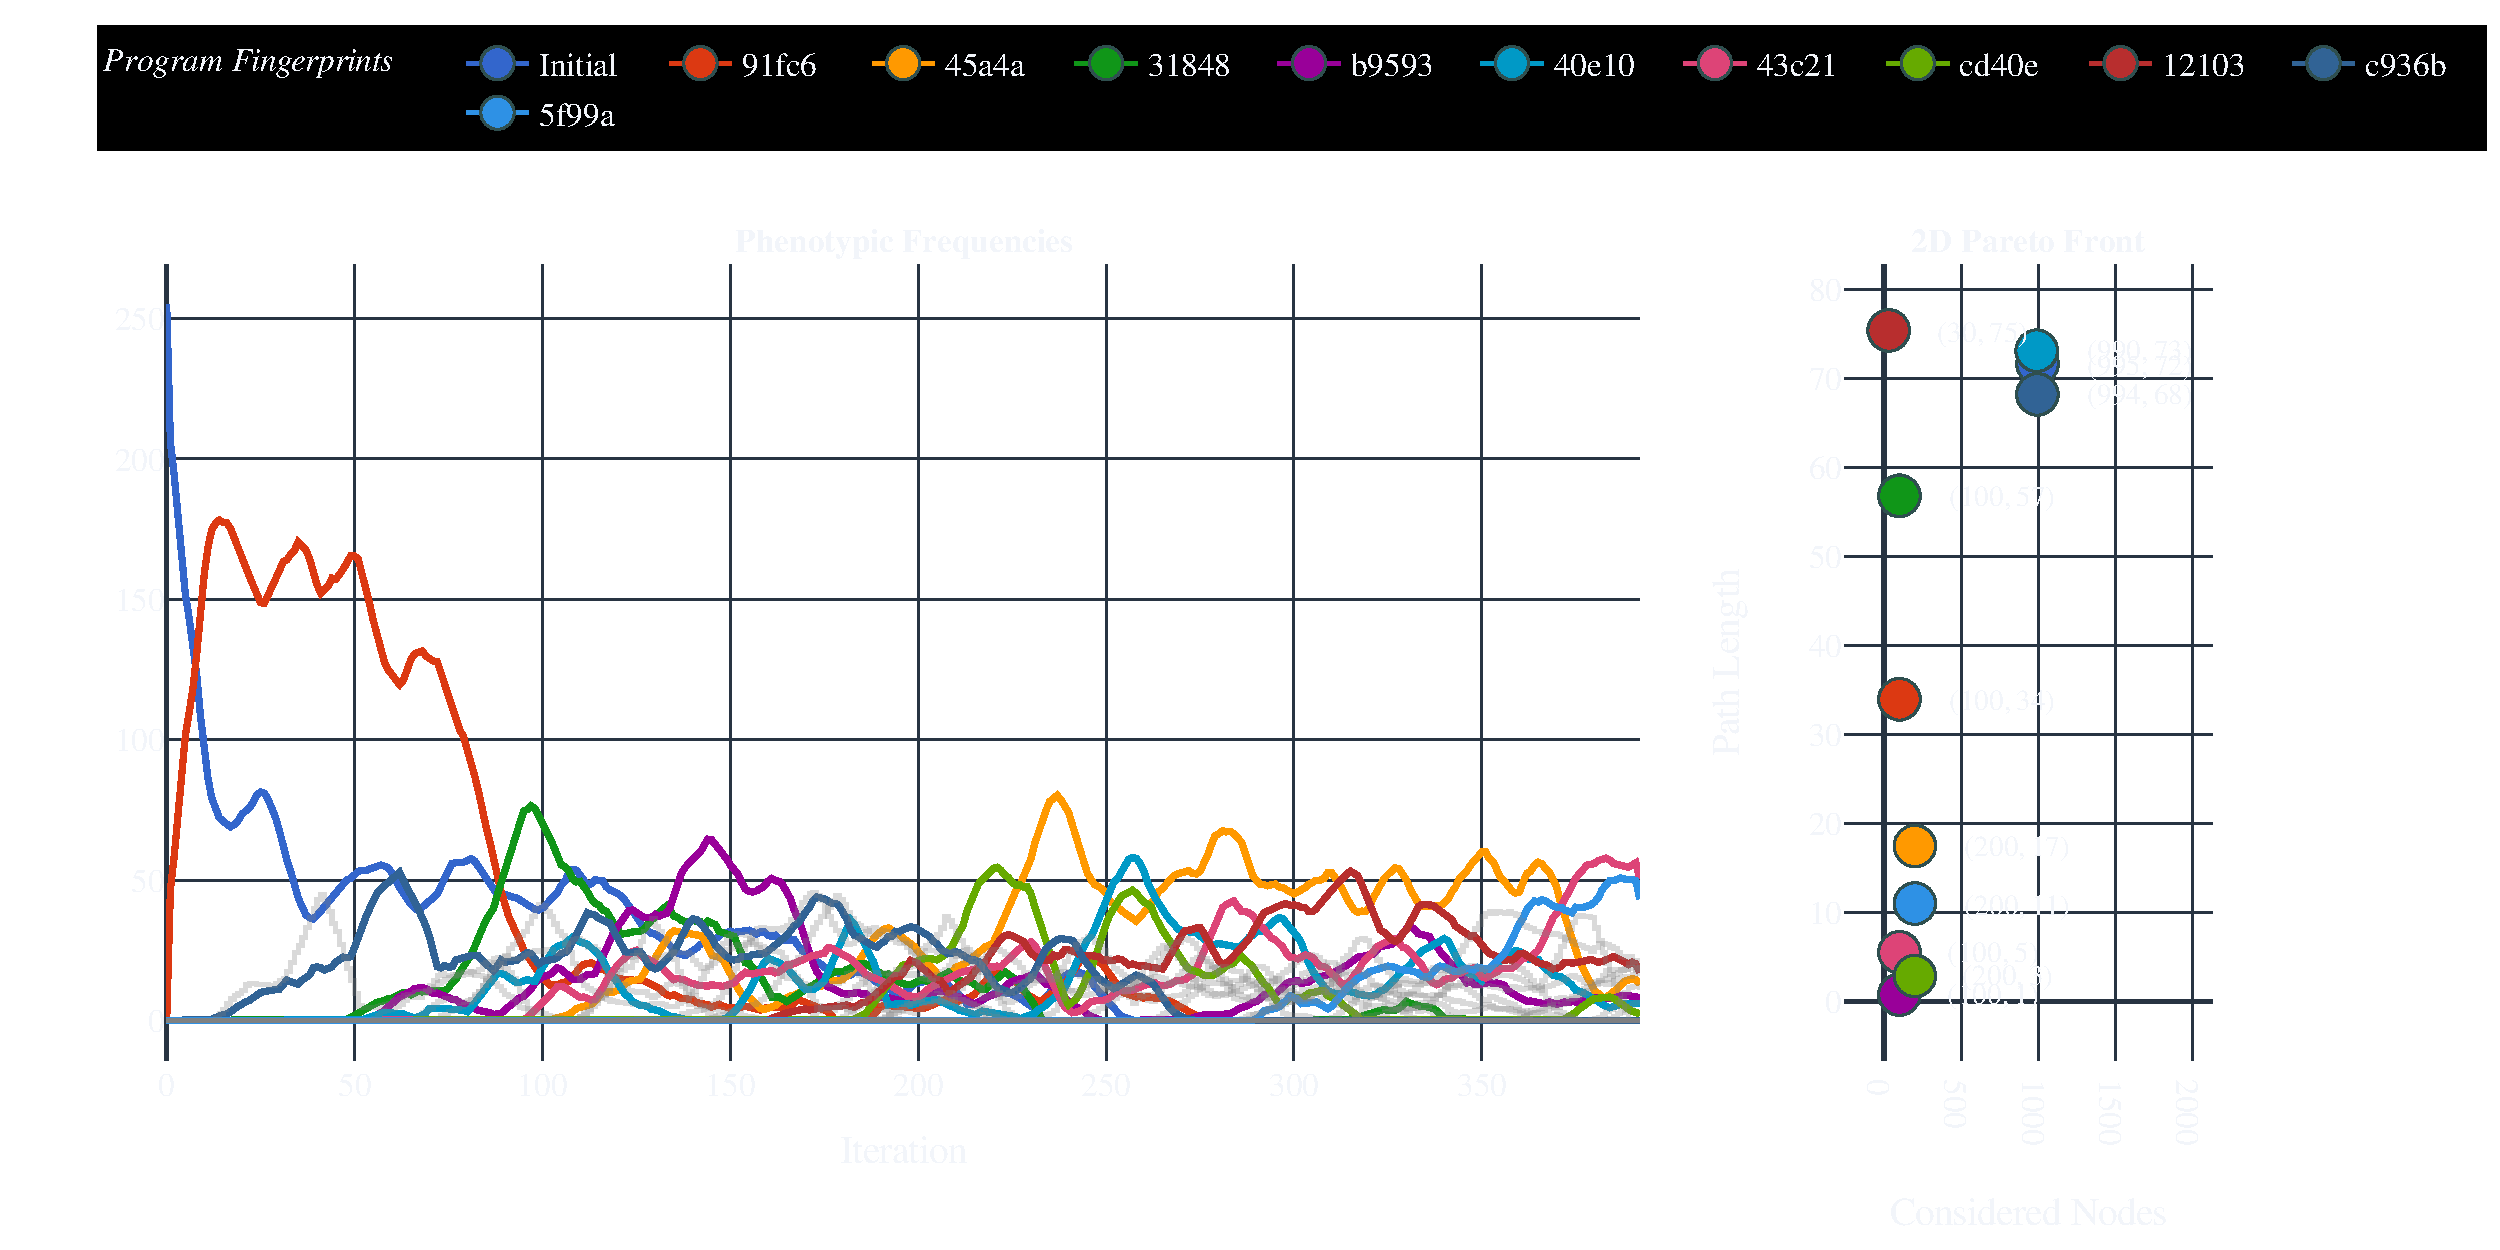
\includegraphics[width=1.0\linewidth, keepaspectratio]{figures/baldurs_pheno_50.pdf}
\end{frame}

\end{document}